\documentclass [11pt,twoside]{article}
\usepackage[utf8]{inputenc}
\usepackage[T1]{fontenc}

%Page margins, header and footer positions
\usepackage{geometry}
 \geometry{
 a4paper,
 total={210mm,297mm},
 left=35mm,
 right=35mm,
 top=30mm,
 bottom=25mm,
 headsep=7mm}

\interfootnotelinepenalty=10000

%To display filling dots in the TOC for all entries
\usepackage[titles]{tocloft}
\renewcommand{\cftsecleader}{\cftdotfill{\cftdotsep}}

%Define new header and footer style
\usepackage{fancyhdr}

\pagestyle{fancy}
\fancyhf{}
\lhead{\color{Gray}{\small{Cracker by Febbo Leonardo, Ferreri Elisabetta}}}
\rfoot{\textcolor{Gray}{\thepage}}
\renewcommand{\headrulewidth}{0pt}

%PACKAGES
\usepackage{pifont}

\newcommand{\supported}{\ding{52}\xspace}
\newcommand{\unsupported}{\ding{55}\xspace}
\newcommand{\partsupported}{\textcolor{black!40}{\ding{52}}\xspace}
\newcommand{\lowsupported}{\textcolor{black!20}{\ding{52}}\xspace}
\newcommand{\unknowsupported}{\textbf{?}\xspace}

%Font: Times
\usepackage{times}
%Change monospaced font
\renewcommand{\ttdefault}{lmtt}

%tables
\usepackage{tabu}
\usepackage{tabularx}
\usepackage{ltablex}
\usepackage{longtable}
\usepackage{float} % To allow the use of H modifier in long tables

%landscape mode
\usepackage{pdflscape}
\usepackage{rotating}
\usepackage{caption}

%make landscape mode be sensitive to even and odd pages
%start
\def\myrotate{\ifodd\c@page\else-\fi 90}
\makeatletter
\global\let\orig@begin@landscape=\landscape%
\global\let\orig@end@landscape=\endlandscape%
\gdef\@true{1}
\gdef\@false{0}
\gdef\landscape{%
    \global\let\within@landscape=\@true%
    \orig@begin@landscape%
}%
\gdef\endlandscape{%
    \orig@end@landscape%
    \global\let\within@landscape=\@false%
}%
\@ifpackageloaded{pdflscape}{%
    \gdef\pdf@landscape@rotate{\PLS@Rotate}%
}{
    \gdef\pdf@landscape@rotate#1{}%
}
\let\latex@outputpage\@outputpage
\def\@outputpage{
    \ifx\within@landscape\@true%
        \if@twoside%
            \ifodd\c@page%
                \gdef\LS@rot{\setbox\@outputbox\vbox{%
                    \pdf@landscape@rotate{-90}%
                    \hbox{\rotatebox{90}{\hbox{\rotatebox{180}{\box\@outputbox}}}}}%
                }%
            \else%
                \gdef\LS@rot{\setbox\@outputbox\vbox{%
                    \pdf@landscape@rotate{+90}%
                    \hbox{\rotatebox{90}{\hbox{\rotatebox{0}{\box\@outputbox}}}}}%
                }%
            \fi%
        \else%
            \gdef\LS@rot{\setbox\@outputbox\vbox{%
                \pdf@landscape@rotate{+90}%
                \hbox{\rotatebox{90}{\hbox{\rotatebox{0}{\box\@outputbox}}}}}%
            }%
        \fi%
    \fi%
    \latex@outputpage%
}
\makeatother
%end

%graphics
\usepackage{graphicx}
\usepackage[dvipsnames, table]{xcolor}
%If you upload images from PC, you need to insert code for the path here (different for Windows and Unix OS)

%References
%\usepackage{xpatch}
%\usepackage[backend=biber, style=numeric, citestyle=numeric, sorting=none]{biblatex}
%\addbibresource{main.bib}

%Other
\usepackage{ifthen}
\usepackage{xspace}
\usepackage{enumitem}
\usepackage{amssymb}
\usepackage[pdftex, colorlinks]{hyperref}
\newcommand{\comment}[1]{{\color{Red}$\blacktriangleright$ Comment: #1 $\blacktriangleleft$}}


% Some utilities\ldots
\usepackage{soul}
\usepackage{tikz}

\usetikzlibrary{calc}
\usetikzlibrary{decorations.pathmorphing}


\makeatletter

\newcommand{\defhighlighter}[3][]{%
  \tikzset{every highlighter/.style={color=#2, fill opacity=#3, #1}}%
}

\defhighlighter{yellow}{.5}

\newcommand{\highlight@DoHighlight}{
  \fill [ decoration = {random steps, amplitude=1pt, segment length=15pt}
        , outer sep = -15pt, inner sep = 0pt, decorate
       , every highlighter, this highlighter ]
        ($(begin highlight)+(0,8pt)$) rectangle ($(end highlight)+(0,-3pt)$) ;
}

\newcommand{\highlight@BeginHighlight}{
  \coordinate (begin highlight) at (0,0) ;
}

\newcommand{\highlight@EndHighlight}{
  \coordinate (end highlight) at (0,0) ;
}

\newdimen\highlight@previous
\newdimen\highlight@current

\DeclareRobustCommand*\highlight[1][]{%
  \tikzset{this highlighter/.style={#1}}%
  \SOUL@setup
  %
  \def\SOUL@preamble{%
    \begin{tikzpicture}[overlay, remember picture]
      \highlight@BeginHighlight
      \highlight@EndHighlight
    \end{tikzpicture}%
  }%
  %
  \def\SOUL@postamble{%
    \begin{tikzpicture}[overlay, remember picture]
      \highlight@EndHighlight
      \highlight@DoHighlight
    \end{tikzpicture}%
  }%
  %
  \def\SOUL@everyhyphen{%
    \discretionary{%
      \SOUL@setkern\SOUL@hyphkern
      \SOUL@sethyphenchar
      \tikz[overlay, remember picture] \highlight@EndHighlight ;%
    }{%
    }{%
      \SOUL@setkern\SOUL@charkern
    }%
  }%
  %
  \def\SOUL@everyexhyphen##1{%
    \SOUL@setkern\SOUL@hyphkern
    \hbox{##1}%
    \discretionary{%
      \tikz[overlay, remember picture] \highlight@EndHighlight ;%
    }{%
    }{%
      \SOUL@setkern\SOUL@charkern
    }%
  }%
  %
  \def\SOUL@everysyllable{%
    \begin{tikzpicture}[overlay, remember picture]
      \path let \p0 = (begin highlight), \p1 = (0,0) in \pgfextra
        \global\highlight@previous=\y0
        \global\highlight@current =\y1
      \endpgfextra (0,0) ;
      \ifdim\highlight@current < \highlight@previous
        \highlight@DoHighlight
        \highlight@BeginHighlight
      \fi
    \end{tikzpicture}%
    \the\SOUL@syllable
    \tikz[overlay, remember picture] \highlight@EndHighlight ;%
  }%
  \SOUL@
}

\makeatother

% Common abbrev. are set as commands to ensure proper spacing after the dot
\RequirePackage{xspace}
\newcommand{\ie}{i.e.\@\xspace}
\newcommand{\aka}{a.k.a.\@\xspace}
\newcommand{\Ie}{I.e.\@\xspace}
\newcommand{\cf}{cf.\@\xspace}
\newcommand{\Cf}{Cf.\@\xspace}
\newcommand{\eg}{e.g.\@\xspace}
\newcommand{\Eg}{E.g.\@\xspace}
\newcommand{\etal}{et al.\@\xspace}
\newcommand{\etc}{etc.\@\xspace}
\newcommand{\wrt}{w.r.t.\@\xspace}
\newcommand{\Wrt}{W.r.t.\@\xspace}



\date{}


\usepackage{listings}
\usepackage{color}

\definecolor{dkgreen}{rgb}{0,0.6,0}
\definecolor{gray}{rgb}{0.5,0.5,0.5}
\definecolor{mauve}{rgb}{0.58,0,0.82}

\lstset{frame=tb,
  language=Java,
  aboveskip=3mm,
  belowskip=3mm,
  showstringspaces=false,
  columns=flexible,
  basicstyle={\small\ttfamily},
  numbers=none,
  numberstyle=\tiny\color{gray},
  keywordstyle=\color{blue},
  commentstyle=\color{dkgreen},
  stringstyle=\color{mauve},
  breaklines=true,
  breakatwhitespace=true,
  tabsize=3
}

\begin{document}

%TITLE PAGE

\begin{titlepage}

%TITLE 

\begin{center}

{\Large{\scshape{Politecnico di Milano}}}
\vspace{6mm}


\includegraphics[scale=0.2]{img/polimi}
\vspace{6mm}

{\Large{\scshape{Design and Implementation of Mobile Applications}}}
\vspace{20mm}


\includegraphics[scale=0.5]{img/logo}
\vspace{8mm}

{\textbf{\Huge{Cracker}}}
\vspace{10mm}

{\textbf{\Large{Design Document}}}
\vspace{25mm}

{\slshape{\Large{by}}} 
\vspace{3mm}

{\slshape{\Large{Leonardo Febbo}}} 
\vspace{3mm}

{\slshape{\Large{Elisabetta Ferreri}}}

\vfill
{\large{February 17, 2020}}

\end{center}

\end{titlepage}

\setcounter{page}{2}


%------------------------------------------------------------------------------------------------------------------------------------------------
\newpage
{
	\hypersetup{linkcolor=black}
	\tableofcontents
}
%------------------------------------------------------------------------------------------------------------------------------------------------
\clearpage
{\section{Introduction}}
\label{sect:introduction}
\subsection{Purpose}
The purpose of this document is to describe the design phases of the realization of the "Cracker" mobile application, with particular attention to the architecture and the user experience. \newline
The main aim of "Cracker" is to help users who read Marvel comics by letting them mark the issues they have read and keeping them up to date with the newest releases by Marvel. \newline
This project is the result of the implementation of the knowledge acquired during the course ”Design and Implementation of Mobile Applications” provided by Politecnico di Milano.


\subsection{Definitions and acronyms}
\subsubsection{Definitions}
\begin{itemize}
\item {\textbf{Framework}}: reusable set of libraries or classes for a software system
\item {\textbf{Issue}}: a single, periodical, magazine-like publication
\item {\textbf{REST}}: a way of providing interoperability between computer systems on the Internet
\item {\textbf{Series}}: a title collecting a variable amount of issues
\item {\textbf{User}}: a person who has performed the login operation successfully
\end{itemize}

\subsubsection{Acronymns}
\begin{itemize}
\item {\textbf{API}}: Application Programming Interface
\item {\textbf{HTTPS}}: HyperText Transfer Protocol Secure
\item {\textbf{JSON}}: JavaScript Object Notation
\item {\textbf{MVC}}: Model - View - Controller
\item {\textbf{URL}}: Uniform Resource Locator
\end{itemize}


\subsection{Scope}
Cracker has been developed for users who regularly read Marvel comics and want to keep track of the series they are reading and the new issues that are released every week by the American publishing house. Similar apps already exist for other types of media, such as tv shows and movies, but none of them have comics as their focus. Keeping the possible needs of the users in mind, six main screens have been found of interest for our application:
\begin{itemize}
\item {\textbf{Issue}}: screen displaying information about a selected issue
\item {\textbf{Series}}: screen displaying information about a selected series
\item {\textbf{Up Next}}: list of issues to be published in the current week, in the next week and in the current month
\item {\textbf{To Read}}: list of the next issues to read for each of the series the user follows
\item {\textbf{Search}}: search for a series given its name
\item {\textbf{Profile}}: personal information about the user
\end{itemize}


\subsection{Framework}
The development of Cracker was achieved through the use of native iOS SDKs, in particular by using the Swift programming language. This choice allowed greater control of system resources and access to system services, otherwise not possible if using cross-platform frameworks. The purpose is to implement different functionalities and integration with other sites.


\subsection{Functional requirements}
Cracker provides a simple, intuitive and user-friendly interface that allows the users to:
\begin{enumerate}
\item register with a personal e-mail or login with Facebook and Google
\item see information about an issue
\item see information about a series
\item mark series they are reading as {\slshape{following}}
\item select which issues of a series they have read
\item see the next issue not yet read for all the series they are following
\item see the series they are following
\item see statistics on the series they are following
\item see, on a weekly basis, the latest issues of all the series Marvel is publishing
\item search for a specific series, given its name
\end{enumerate}


\subsection{Non-functional requirements}
The application must be able to:
\begin{itemize}
\item run on both iPhone and iPad
\item adapt its written content to the language selected in the device settings (available languages: English, Italian)
\item adapt to different screen sizes
\item keep preferences and status at every start
\end{itemize}


\subsection{Assumptions, dependencies, constraints}
\subsubsection{Assumptions and dependencies}
\begin{itemize}
\item {\textbf{Internet connection}}: the device used by the user disposes of an Internet connection and a sufficient bandwidth to use the application
\item {\textbf{API availability}}: the API provided by third part's services are always available
\item{\textbf{No privileged users}}: there are no privileged users or administrators with particular functions
\item{\textbf{No user connections}}: every user is independent from the others
\end{itemize}

\subsubsection{Constraints}
\begin{itemize}
\item{\textbf{Hardware limitations}}: our application runs on every mobile device like smartphones and tablets; therefore, as the app consumes a low amount of RAM, the only hardware constraint for the users is to have a mid-range device
\item{\textbf{Parallel operations}}: the application must be able to handle multiple parallel requests with high reactivity
\end{itemize}





%------------------------------------------------------------------------------------------------------------------------------------------------
\clearpage
{\section{Architecture}}
\label{sect:architecture}
\subsection{Overview}
In this section we describe the architectural design of our system, the main components and their interactions. \\
The system will be described starting with high-level components. Then a more detailed description is provided for the client and the database structure, including the architectural patterns applied.

\subsection{High level components}
The main high level components of our system are:
\begin{itemize}
\item {\textbf{Client}}: this component is responsible for the visualization of data (front-end) and for the management of requests and replies to and from the services providing data to the system.
\item {\textbf{Firebase}}: this component is responsible for the storage of the permanent data of the users and for the registration and login of users; we use the services provided by Firebase to manage these data.
\item {\textbf{Marvel APIs}}: we use the APIs provided by Marvel in order to always have complete and up-to-date data on comics.
\item {\textbf{Facebook}}: used for the login procedure.
\item {\textbf{Google}}: used for the login procedure.
\end{itemize}

\vspace{3mm}

\begin{figure}[h]
\centering
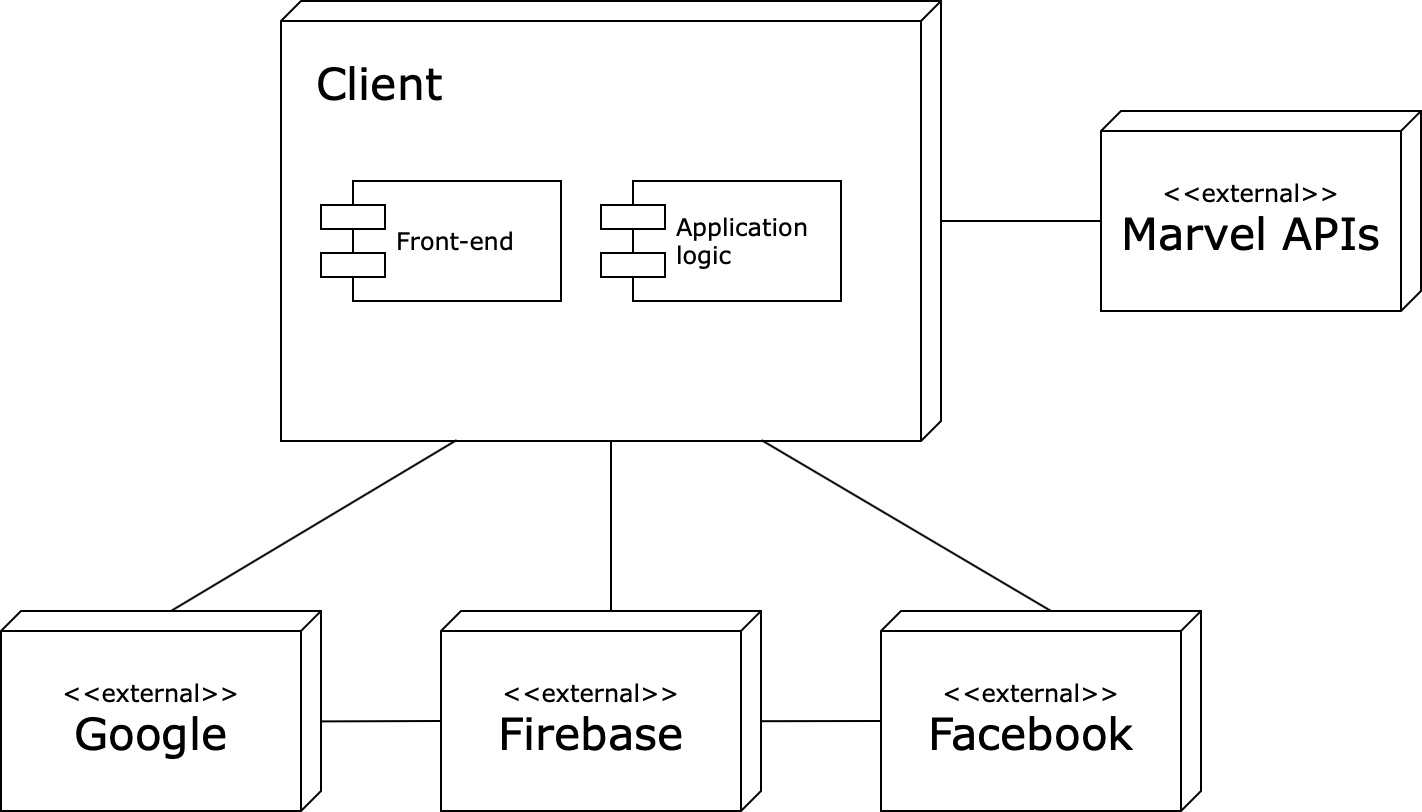
\includegraphics[width=\textwidth]{img/components}
\caption{High Level Component View}
\end{figure}

\clearpage

\subsection{Client}
For the implementation of the application we have chosen a mobile back-end, that is a client architecture. This choice was made mainly because the application does not interface with other users and because for various services it uses third-party APIs. Communication with third-party services is based on HTTPS REST requests, in particular through GET requests.
The client uses the traditional MVC pattern:
\begin{itemize}
\item Model: this package contains all the classes representing data to be shown to the single user, taken by the Controller and published by the View.
\item View: this package contains all the components that display data to the user and interact with him.
\item Controller: this package contains all the objects in charge to interact between one or more view objects of the application and one or more model objects.
\end{itemize}

\subsection{Database}
Since the application receives all the necessary data from external services through the API, the only data that has to be saved is the information about the user, the series that he follows and the comics he has read. Moreover, since there is no interaction between the different users, this data is saved on the Cloud Firestore on Firebase Platform to guarantee ACID properties. The database interacts only with the application layer. The security restriction will be implemented to guarantee the user privacy from unauthorized users. The communication between the database and application tier has to be encrypted. The access to the data has to be guaranteed only to the authorized user for that data.

\begin{figure}[h]
\centering
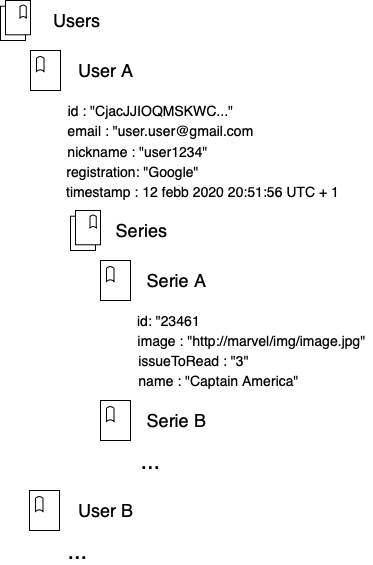
\includegraphics[scale=0.5]{img/DB}
\caption{Database Cloud FIrestore}
\end{figure}

\clearpage

The E / R model of the data collected through the API together with the user data saved on the firebase is as follows:


\begin{figure}[h]
\centering
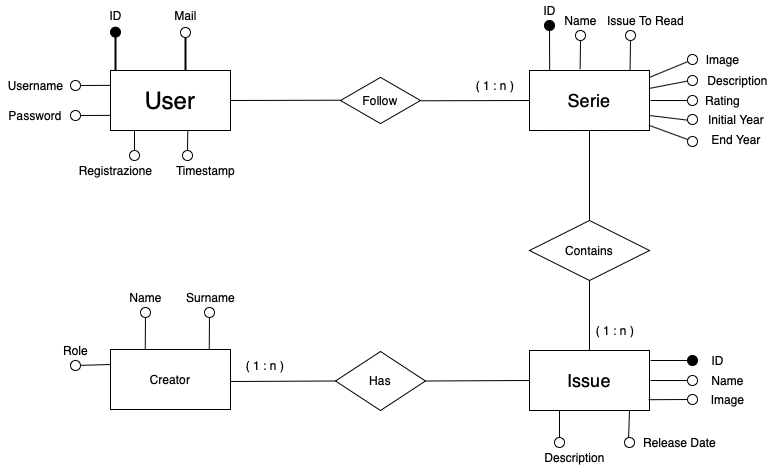
\includegraphics[width=\textwidth]{img/ER}
\caption{E/R Diagram}
\end{figure}




%------------------------------------------------------------------------------------------------------------------------------------------------
\clearpage
{\section{External Services and Libraries}}
\label{sect:extservices}
Cracker application uses Marvel Developer API in order to provide the user all the services. The SwiftyJSON component from UIKit was used to parse the JSON data.
\subsection{Facebook SDK}

The Facebook SDK was used to manage the login through Facebook account. When a user wants to authenticate the application makes the call to the Facebook service through:
\begin{lstlisting}
func loginButton(_ loginButton: FBLoginButton, didCompleteWith result: LoginManagerLoginResult?, error: Error?) {
	if let error = error {
		print(error.localizedDescription)
		return
	}else{
		let credential = FacebookAuthProvider.credential(withAccessToken: AccessToken.current!.tokenString)
		// then sign in through firebase with this credentials
	} 
}
\end{lstlisting}

This method is used to send the user on Facebook for the authentication; once authenticated the user redirected to ”Cracker” which will store the token provided into Firebase.
The following pods were included to use Facebook:

\begin{lstlisting}
pod 'FacebookCore'
pod 'FacebookLogin'
\end{lstlisting}

\clearpage
  
  
\subsection{Google SDK}
The Google SDK was used to manage the login through Google account. When a user wants to authenticate the application makes the call to the Google service through:
\begin{lstlisting}
func sign(_ signIn: GIDSignIn!, didSignInFor user: GIDGoogleUser!, withError error: Error!) {
	if let error = error {
		if (error as NSError).code == GIDSignInErrorCode.hasNoAuthInKeychain.rawValue {
			print("The user has not signed in before or they have since signed out.")
		} else {
			print("\(error.localizedDescription)")
		}
		return
	}else{
		guard let authentication = user.authentication else { return }
		let credential = GoogleAuthProvider.credential(withIDToken: authentication.idToken, accessToken: authentication.accessToken)
		// then sign in through firebase with this credentials
	}
}
\end{lstlisting}
This method is used to send the user on Google for the authentication; once authenti- cated the user redirected to ”Cracker” which will store the token provided into Firebase.
The following pods were included to use Google:
\begin{lstlisting}
pod 'GoogleSignIn'
\end{lstlisting}
    
\clearpage
    
    
\subsection{Firebase SDK}
Firebase SDKs are used to access the database, to login with email and password and to save other authentication through Facebook and Google.
\begin{lstlisting}
Auth.auth().signIn(with: credential) { (authResult, error) in
	if error == error{
		print("Error Log In Firebase \(error)")
		return
	}else{
		print("Logged In Firebase")
	}
}
\end{lstlisting}

For database access, the components included in the SDKs was used:
\begin{lstlisting}
let user = Firestore.firestore().collection("Users").document("\((Auth.auth().currentUser?.uid)!)")
User.collection("Series").getDocuments() { (querySnapshot, err) in
	if let err = err {
		print("Error getting documents: \(err)")
	} else {
		print("Collection got")
		...
	}
}
\end{lstlisting}

The following pods were included to use Firebase:
\begin{lstlisting}
pod 'Firebase/Auth'
pod 'Firebase/Firestore'
pod 'Firebase/Analytics'
pod 'FirebaseFirestoreSwift'
\end{lstlisting}


\clearpage

\subsection{Alamofire}
Alamofire is used to send GET requests to the endpoint supplied by Marvel APIs. If the answer is valid, it returns a JSON file that can be parsed.
\begin{lstlisting}
Alamofire.request(url, method: .get, parameters: parameters).responseJSON { response in
	if response.result.isSuccess {
		print("Success! Got the data")
		let json : JSON = JSON(response.result.value!)
	}else {
		print("Error \(String(describing: response.result.error))")
	}
}
\end{lstlisting}
The following pods were included to use Alamofire:
\begin{lstlisting}
pod 'Alamofire'
\end{lstlisting}

\clearpage

\subsection{Marvel Comics API}
The Marvel Comics API is a RESTful service which provides methods for accessing spe- cific resources at canonical URLs and for searching and filtering sets of resources by various criteria. All representations are encoded as JSON objects. All documentation can be found here: https://developer.marvel.com/

\subsubsection{Service Endpoint}
The Marvel Comics API’s base endpoint is http(s)://gateway.marvel.com/

\subsubsection{Resources}
You can access six resource types using the API:
\begin{itemize}
\item {\textbf{Comics}}: individual print and digital comic issues, collections and graphic novels.
\item {\textbf{Comics series}}: sequentially numbered (well, mostly sequentially numbered) groups comics with the same title.
\item {\textbf{Comics stories}}: indivisible, reusable components of comics. For example, the cover from Amazing Fantasy 15 or the origin of Spider-Man story from that comic.
\item {\textbf{Comics events and crossover}}: big, universe-altering storylines.
\item {\textbf{Creators}}: women, men and organizations who create comics.
\item {\textbf{Characters}}: the women, men, organizations, alien species, deities, animals, non- corporeal entities, trans-dimensional manifestations, abstract personifications, and green amorphous blobs which occupy the Marvel Universe (and various alternate universes, timelines and altered realities therein).
\end{itemize}

Results returned by the API endpoints have the same general format, no matter which entity type the endpoint returns. Every successful call will return a wrapper object, which contains metadata about the call and a container object, which displays pagination information and an array of the results returned by this call. This pattern is consistent even if you are requesting a single object.


Putting it together, a typical result will look like this:
\begin{lstlisting}
{
	"code": 200,
	"status": "Ok",
	"etag": "f0fbae65eb2f8f28bdeea0a29be8749a4e67acb3",
	"data": {
		"offset": 0,
		"limit": 20,
		"total": 30920,
		"count": 20,
		"results": [{array of objects}}]
	}
}
\end{lstlisting}


\subsubsection{Authentication}
All requests to the APIs must be authenticated using the methods outlined in the request signing and authentication guidelines. Requests which fail authentication generally pass a 401 HTTP code and an error describing the reason for rejection.



























%------------------------------------------------------------------------------------------------------------------------------------------------
\clearpage
{\section{Use Cases}
\label{sect:usecases}
This section describes how actors can interact with Cracker in order to use all the features implemented in the app. The focus of this part is on the front-end and we show the operations that can be performed by the actors without taking care of the system architecture behind the app.

\vspace{6mm}

\subsection{Login}
\begin{figure}[h]
\centering
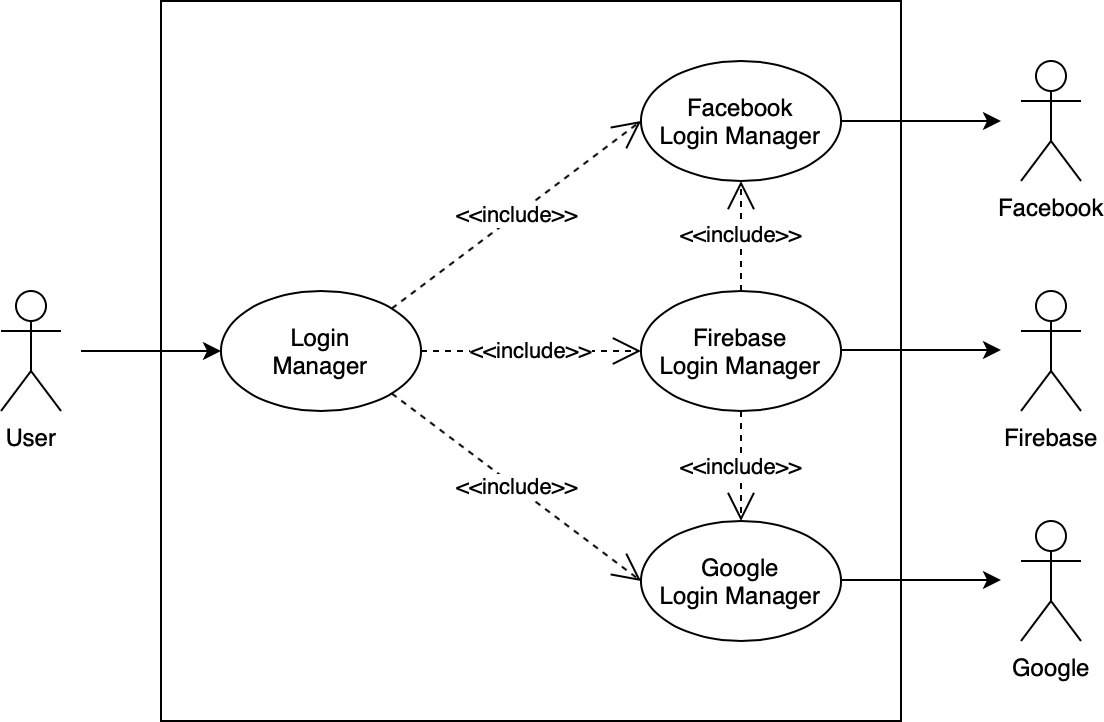
\includegraphics[width=\textwidth]{img/usecases/login}
\end{figure}

\clearpage

{\renewcommand{\arraystretch}{2}
{\begin{center}
\begin{tabular}{ | m{4cm} | m{9cm} | } 
 \hline
 {\centering{\textbf{Name}}} & Login \\
 \hline
 {\centering{\textbf{Actor}}} & User \\
 \hline
 {\centering{\textbf{Entry Condition}}} & Guest with login credentials \\
 \hline
 {\centering{\textbf{Goal}}} & 1 \\
 \hline
 {\centering{\textbf{Event flow}}} & \begin{itemize}[leftmargin=*]
 	\item The user opens the application
	\item The user presses ”Login with Facebook” (or "Login with Google") located in the welcome screen
	\item The user is redirected on Facebook (or Google) to enter credentials
	\item The app logs in through Facebook (or Google)
	\item The app login into Firebase using Facebook (or Google) account 
	\end{itemize} \\	
 \hline
 {\centering{\textbf{Exit condition}}} & Actor becomes Logged User \\
 \hline
 {\centering{\textbf{Exceptions}}} & The user is not connected to the network or he hasn’t a Facebook or Google account \\
 \hline
\end{tabular}
\end{center}}

\clearpage

\subsection{View Up Next}
\begin{figure}[h]
\centering
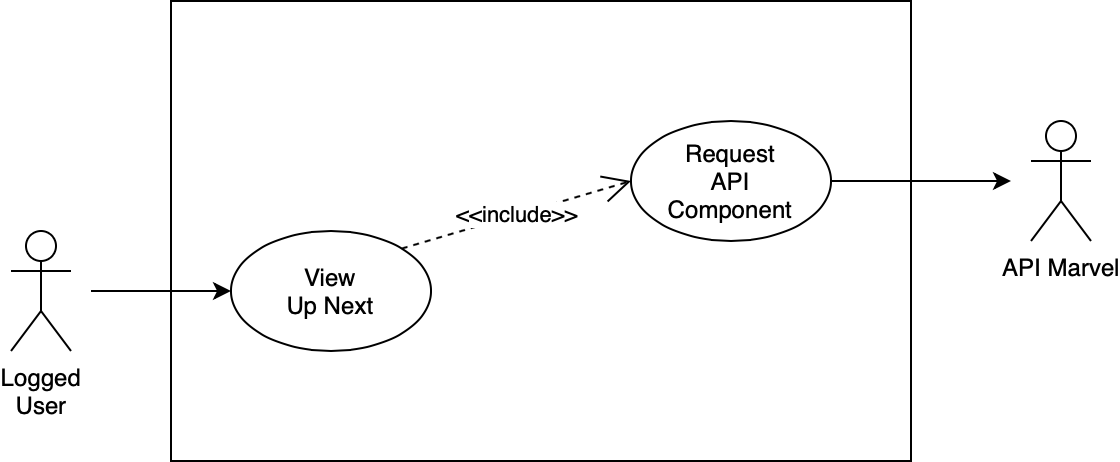
\includegraphics[width=\textwidth]{img/usecases/viewupnext}
\end{figure}

{\renewcommand{\arraystretch}{2}
{\begin{center}
\begin{tabular}{ | m{4cm} | m{9cm} | } 
 \hline
 {\centering{\textbf{Name}}} & View Up Next \\
 \hline
 {\centering{\textbf{Actor}}} & Logged User \\
 \hline
 {\centering{\textbf{Entry Condition}}} & The user logged in correctly \\
 \hline
 {\centering{\textbf{Goal}}} & 9 \\
 \hline
 {\centering{\textbf{Event flow}}} & \begin{itemize}[leftmargin=*]
 	\item The user opens the application
	\item The user presses on the "Up Next" tab located on the Tab Bar
	\item The app shows the upcoming issues divided by being published this week, next week, this month
	\end{itemize} \\	
 \hline
 {\centering{\textbf{Exit condition}}} & The user reads the titles of the upcoming issues \\
 \hline
 {\centering{\textbf{Exceptions}}} & The user is not connected to the network so he cannot send a request to read the titles of the upcoming issues \\
 \hline
\end{tabular}
\end{center}}

\clearpage

\subsection{View To Read}
\begin{figure}[h]
\centering
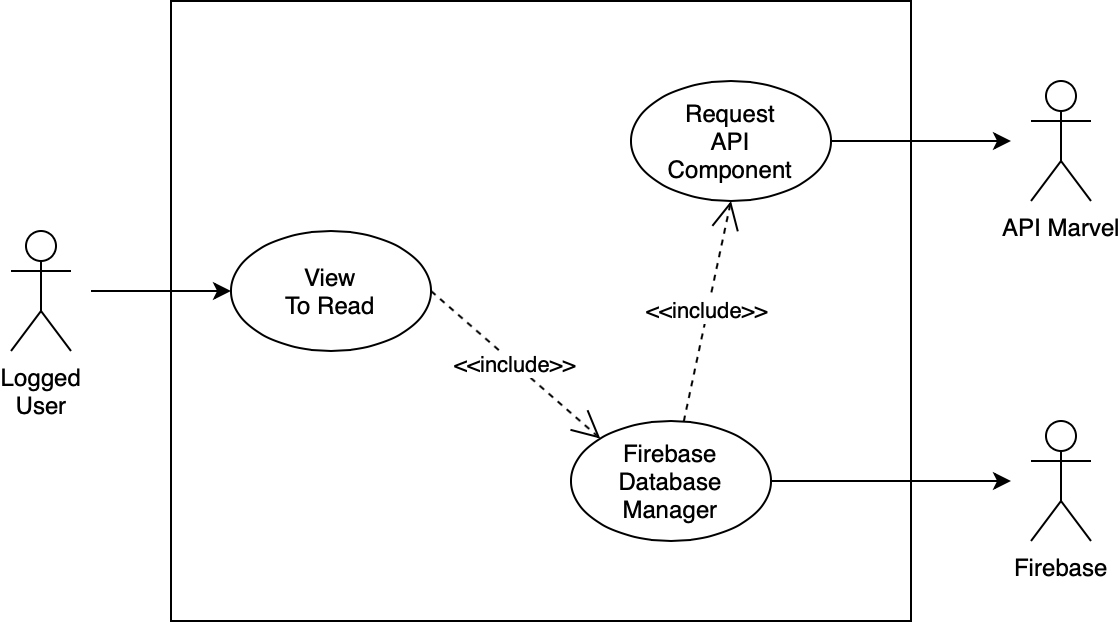
\includegraphics[width=\textwidth]{img/usecases/viewtoread}
\end{figure}

{\renewcommand{\arraystretch}{2}
{\begin{center}
\begin{tabular}{ | m{4cm} | m{9cm} | } 
 \hline
 {\centering{\textbf{Name}}} & View To Read \\
 \hline
 {\centering{\textbf{Actor}}} & Logged User \\
 \hline
 {\centering{\textbf{Entry Condition}}} & The user logged in correctly \\
 \hline
 {\centering{\textbf{Goal}}} & 6 \\
 \hline
 {\centering{\textbf{Event flow}}} & \begin{itemize}[leftmargin=*]
 	\item The user opens the application
	\item The user presses on the "To Read" tab located on the Tab Bar
	\item The app shows the next issue to read for all the series that the user is following
	\end{itemize} \\	
 \hline
 {\centering{\textbf{Exit condition}}} & The user sees the covers of the next issues he has to read \\
 \hline
 {\centering{\textbf{Exceptions}}} & The user is not connected to the network so he cannot send a request to get the next issues he has to read \\
 \hline
\end{tabular}
\end{center}}

\clearpage

\subsection{View Issue}
\begin{figure}[h]
\centering
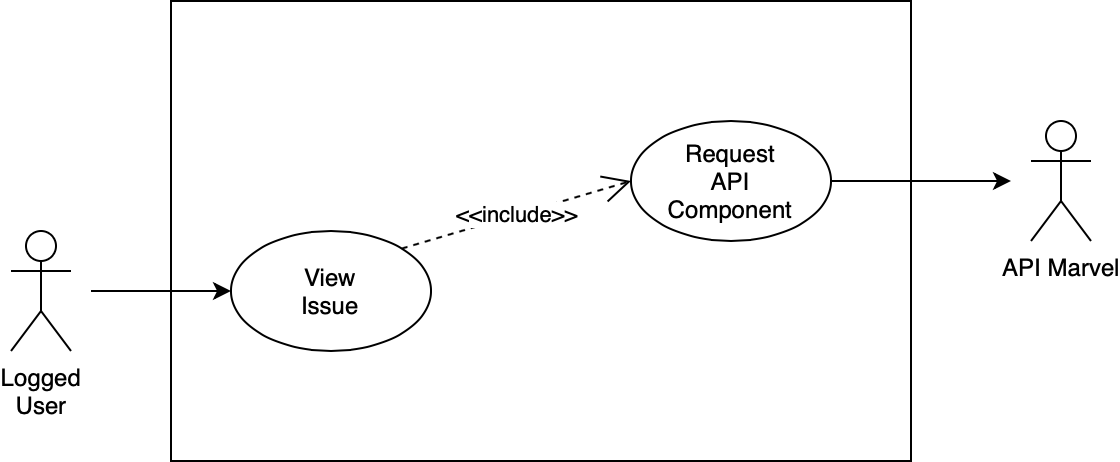
\includegraphics[width=\textwidth]{img/usecases/viewissue}
\end{figure}

{\renewcommand{\arraystretch}{2}
{\begin{center}
\begin{tabular}{ | m{4cm} | m{9cm} | } 
 \hline
 {\centering{\textbf{Name}}} & View Issue \\
 \hline
 {\centering{\textbf{Actor}}} & Logged User \\
 \hline
 {\centering{\textbf{Entry Condition}}} & The user logged in correctly \\
 \hline
 {\centering{\textbf{Goal}}} & 9 \\
 \hline
 {\centering{\textbf{Event flow}}} & \begin{itemize}[leftmargin=*]
 	\item The user opens the application and navigates through some screens
	\item The user presses on the button representing an issue in one of the screen where such a button is present
	\item The app shows the most important information about the issue
	\end{itemize} \\	
 \hline
 {\centering{\textbf{Exit condition}}} & The user reads the information about the issue \\
 \hline
 {\centering{\textbf{Exceptions}}} & The user is not connected to the network so he cannot send a request to get the information about the issue \\
 \hline
\end{tabular}
\end{center}}

\clearpage

\subsection{View Series}
\begin{figure}[h]
\centering
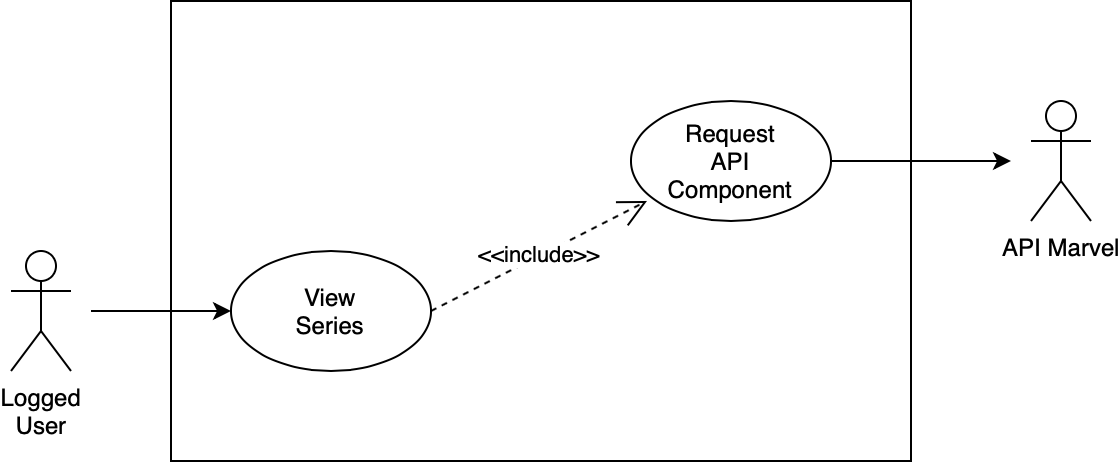
\includegraphics[width=\textwidth]{img/usecases/viewseries}
\end{figure}

{\renewcommand{\arraystretch}{2}
{\begin{center}
\begin{tabular}{ | m{4cm} | m{9cm} | } 
 \hline
 {\centering{\textbf{Name}}} & View Series \\
 \hline
 {\centering{\textbf{Actor}}} & Logged User \\
 \hline
 {\centering{\textbf{Entry Condition}}} & The user logged in correctly \\
 \hline
 {\centering{\textbf{Goal}}} & 9 \\
 \hline
 {\centering{\textbf{Event flow}}} & \begin{itemize}[leftmargin=*]
 	\item The user opens the application and navigates through some screens
	\item The user presses on the button representing a series in one of the screen where such a button is present
	\item The app shows the most important information about the series
	\end{itemize} \\	
 \hline
 {\centering{\textbf{Exit condition}}} & The user reads the information about the series \\
 \hline
 {\centering{\textbf{Exceptions}}} & The user is not connected to the network so he cannot send a request to get the information about the series \\
 \hline
\end{tabular}
\end{center}}

\clearpage

\subsection{Mark Issue as Read}
\begin{figure}[h]
\centering
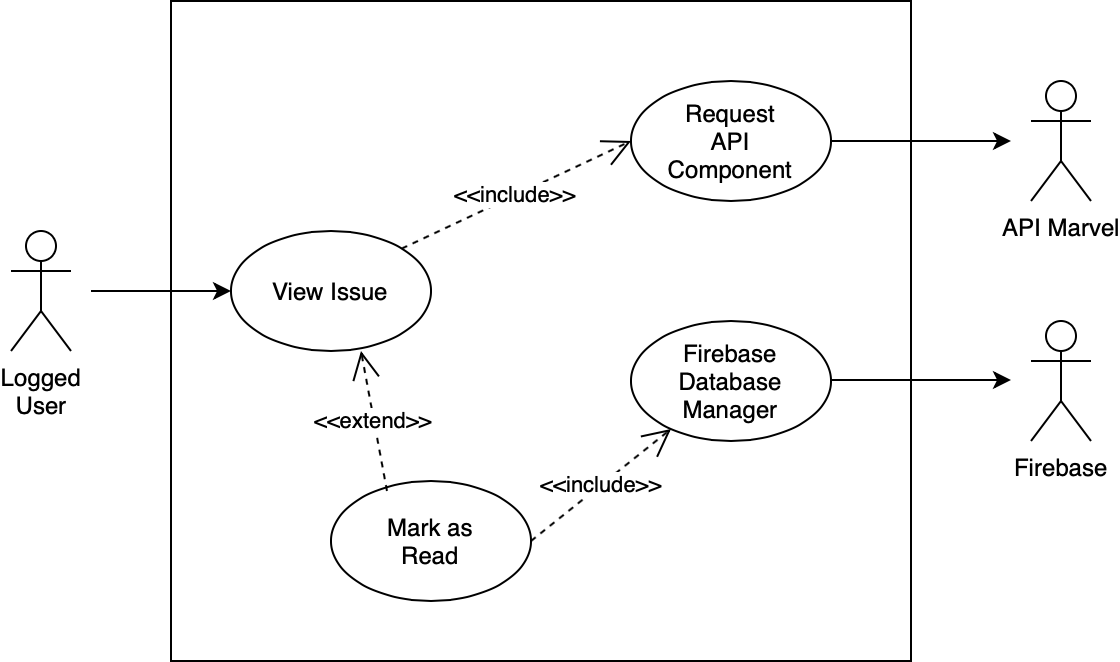
\includegraphics[width=\textwidth]{img/usecases/readissue}
\end{figure}

{\renewcommand{\arraystretch}{2}
{\begin{center}
\begin{tabular}{ | m{4cm} | m{9cm} | } 
 \hline
 {\centering{\textbf{Name}}} & Mark Issue as Read \\
 \hline
 {\centering{\textbf{Actor}}} & Logged User \\
 \hline
 {\centering{\textbf{Entry Condition}}} & The user logged in correctly \\
 \hline
 {\centering{\textbf{Goal}}} & 9 \\
 \hline
 {\centering{\textbf{Event flow}}} & \begin{itemize}[leftmargin=*]
 	\item The user opens the application and navigates through some screens, reaching one with information about an issue
	\item The user presses on the "Mark as read" button 
	\item The app records the action and updates the text of the button to "Mark as unread"
	\end{itemize} \\	
 \hline
 {\centering{\textbf{Exit condition}}} & The user marked an issue as read \\
 \hline
 {\centering{\textbf{Exceptions}}} & The user is not connected to the network so he cannot send a request to mark an issue as read \\
 \hline
\end{tabular}
\end{center}}

\clearpage

\subsection{Follow a Series}
\begin{figure}[h]
\centering
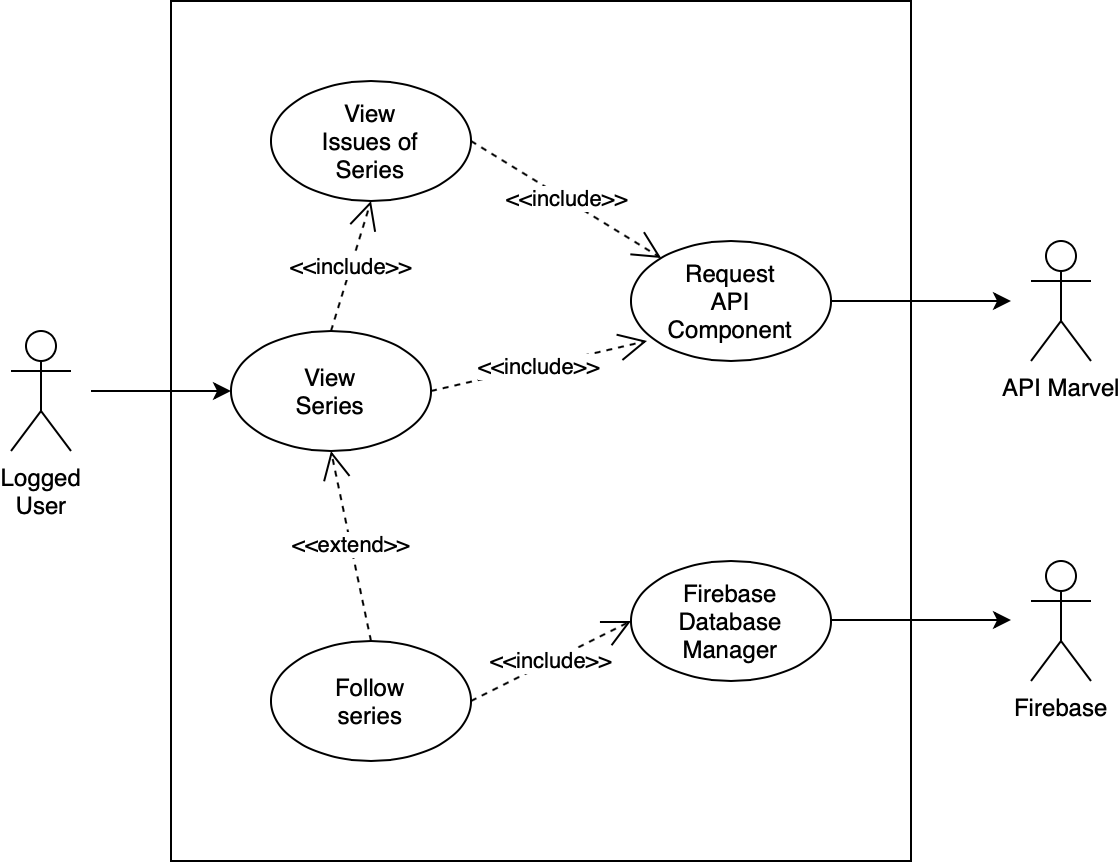
\includegraphics[width=\textwidth]{img/usecases/followseries}
\end{figure}

{\renewcommand{\arraystretch}{2}
{\begin{center}
\begin{tabular}{ | m{4cm} | m{9cm} | } 
 \hline
 {\centering{\textbf{Name}}} & Follow a Series \\
 \hline
 {\centering{\textbf{Actor}}} & Logged User \\
 \hline
 {\centering{\textbf{Entry Condition}}} & The user logged in correctly \\
 \hline
 {\centering{\textbf{Goal}}} & 9 \\
 \hline
 {\centering{\textbf{Event flow}}} & \begin{itemize}[leftmargin=*]
 	\item The user opens the application and navigates through some screens, reaching one with information about a series
	\item The user presses on the "Follow this series" button 
	\item The app records the action and updates the text of the button to "Unfollow this series"
	\end{itemize} \\	
 \hline
 {\centering{\textbf{Exit condition}}} & The user followed a series \\
 \hline
 {\centering{\textbf{Exceptions}}} & The user is not connected to the network so he cannot send a request to follow the series \\
 \hline
\end{tabular}
\end{center}}


\clearpage

\subsection{Search a Series}
\begin{figure}[h]
\centering
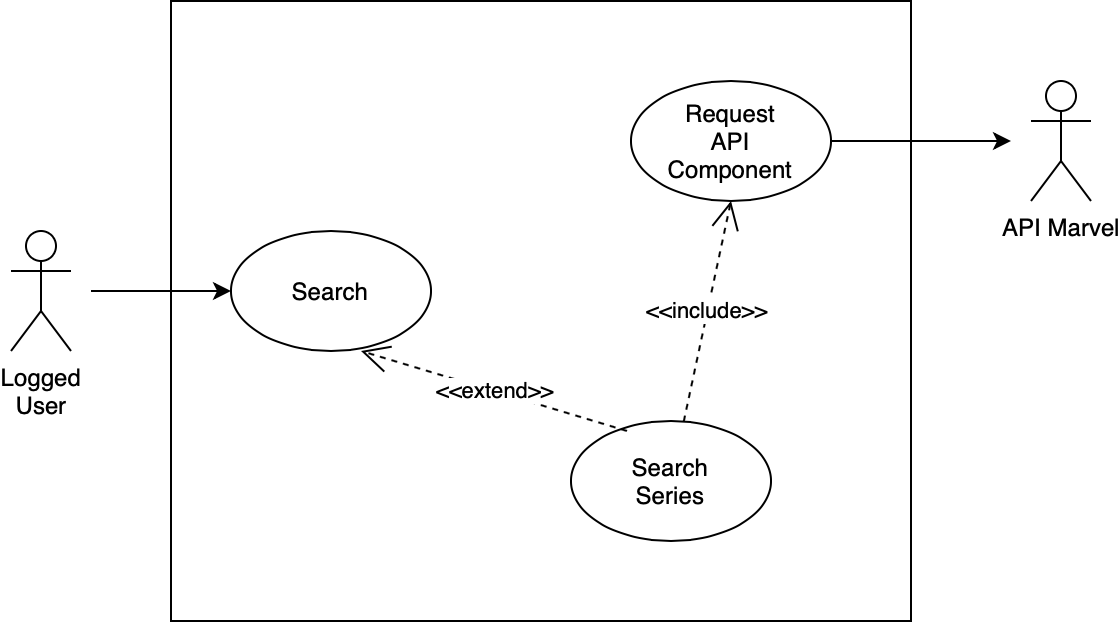
\includegraphics[width=\textwidth]{img/usecases/search}
\end{figure}

{\renewcommand{\arraystretch}{2}
{\begin{center}
\begin{tabular}{ | m{4cm} | m{9cm} | } 
 \hline
 {\centering{\textbf{Name}}} & Search a Series \\
 \hline
 {\centering{\textbf{Actor}}} & Logged User \\
 \hline
 {\centering{\textbf{Entry Condition}}} & The user logged in correctly \\
 \hline
 {\centering{\textbf{Goal}}} & 9 \\
 \hline
 {\centering{\textbf{Event flow}}} & \begin{itemize}[leftmargin=*]
 	\item The user opens the application
	\item The user presses on the "Search" tab located on the Tab Bar
	\item The app show a search bar
	\item The user presses on the search bar and types the name of a series
	\item The app shows the series whose name matches the one written by the user
	\end{itemize} \\	
 \hline
 {\centering{\textbf{Exit condition}}} & The user sees a list of series that match his input \\
 \hline
 {\centering{\textbf{Exceptions}}} & The user is not connected to the network so he cannot send a request to search for series \\
 \hline
\end{tabular}
\end{center}}



%------------------------------------------------------------------------------------------------------------------------------------------------
\clearpage
{\section{Sequence Diagrams}}
\label{sect:sequence}
In order to explain our work and facilitate further implementations we have decided to show the logical flows aimed to create some features. The sequence diagrams will describe the interactions between the different parts of the system and the user.

\vspace{8mm}

\subsection{Login}
The ”Login” procedure starts when the user opens the app for the first time or whenever he logs out. The user can choose to be redirected to either Facebook or Google to complete the procedure. Immediately after logging on Facebook or Google the application will log into the Firebase Database. \\
Once this procedure is completed, the system will update the GUI by enabling the available sections.
In the event of an error, the system will show an error message.

\vspace{5mm}

\begin{figure}[h]
\centering
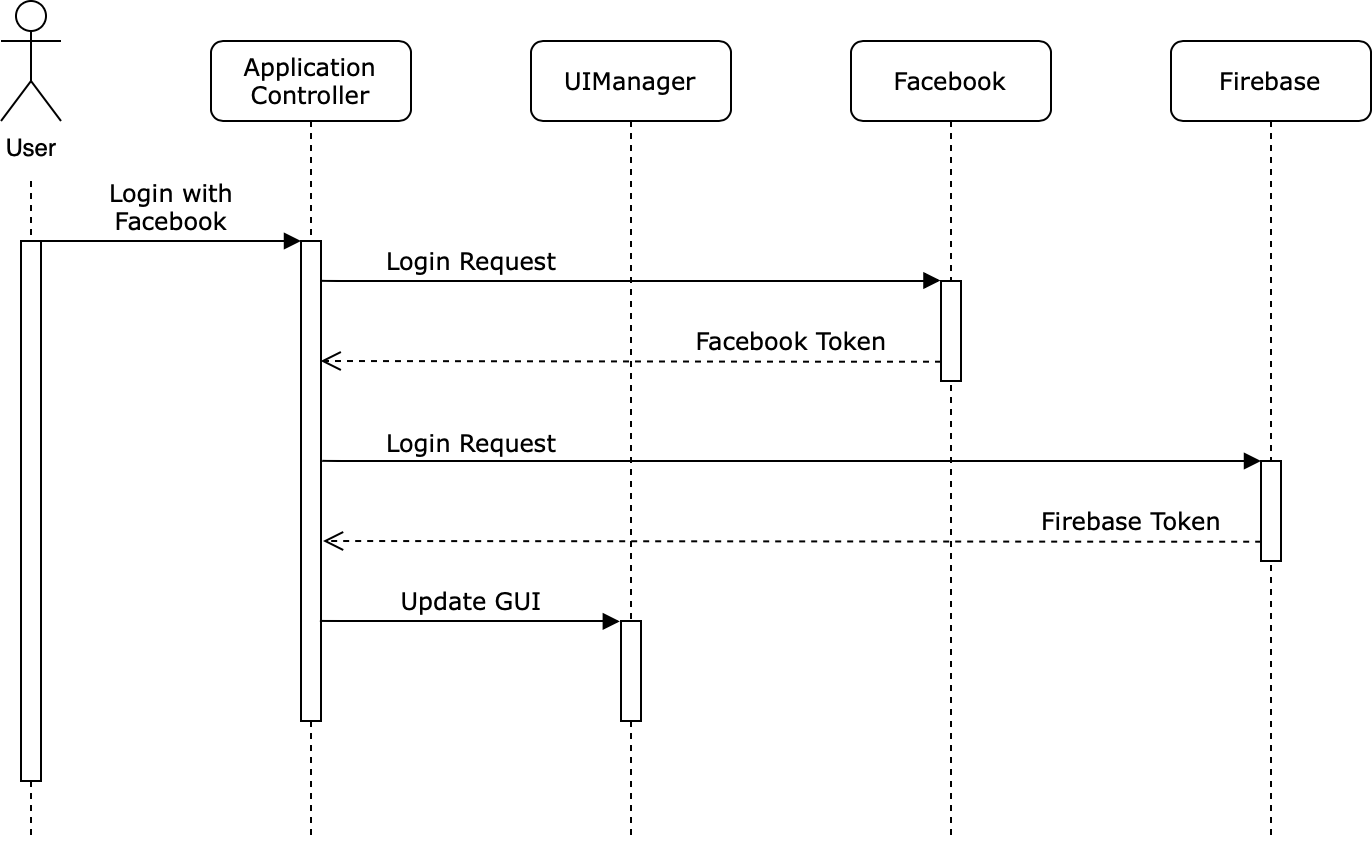
\includegraphics[scale=0.2]{img/seqdiagrams/loginfacebook}
\end{figure}

\begin{figure}[h]
\centering
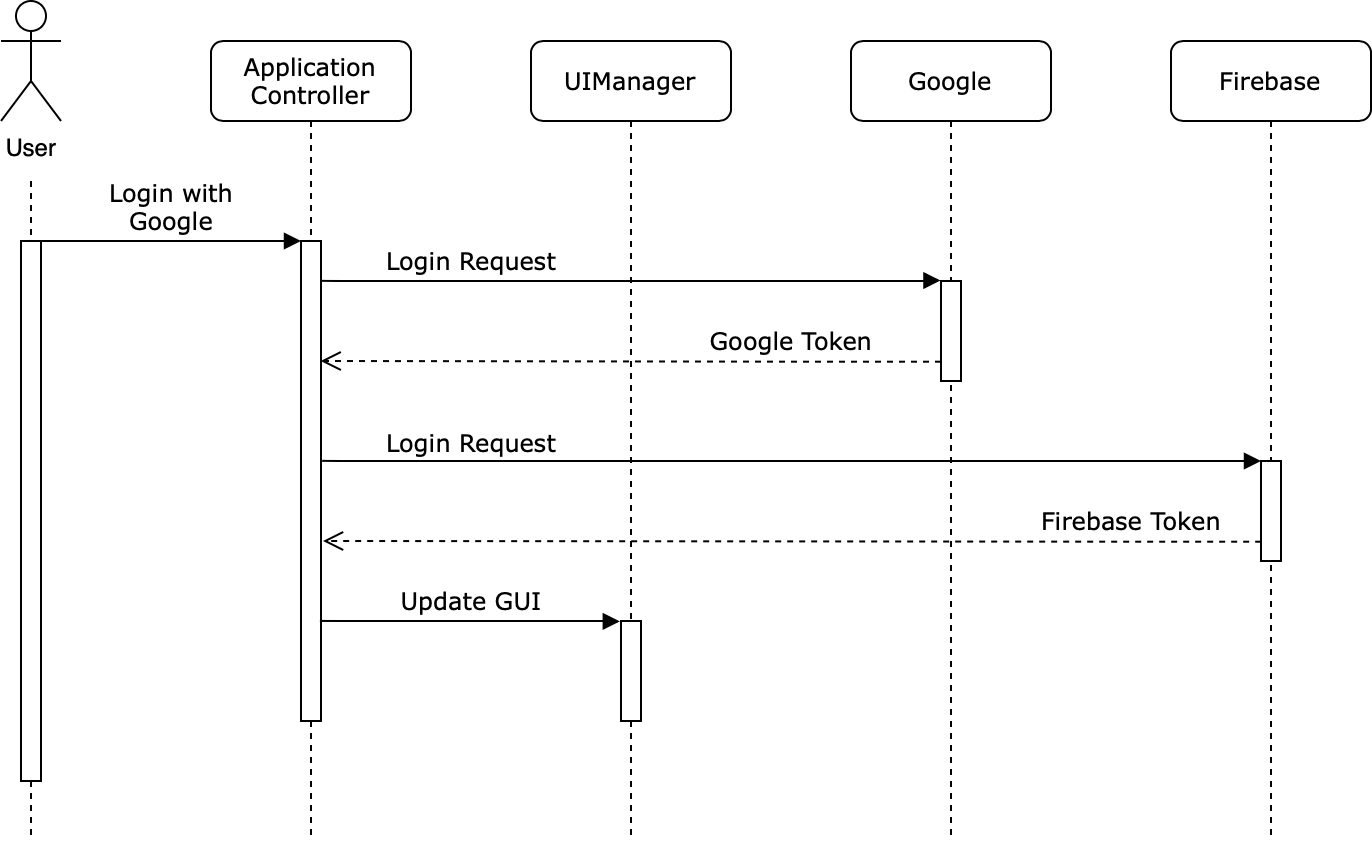
\includegraphics[scale=0.2]{img/seqdiagrams/logingoogle}
\end{figure}

\clearpage

\subsection{View Up Next}
The ”View Up Next” procedure starts when the user opens the application when he's already performed the login or when he presses the ”Up Next” tab in the Tab Bar. The sequence diagram shows the normal procedure. \\
After the user activates the "Up Next" tab, the application will send 3 requests to the ”MarvelAPI” service, one for each of the sections that will be displayed (comics released in the current week, comics released in the following week, comics released in the current month), in order to retrieve the titles of the issues belonging in each of the sections. \\
Once this information is obtained, the Controller will create a UITableViewCell for each issue and insert them into the correct section in a TableView. 

\vspace{5mm}

\begin{figure}[h]
\centering
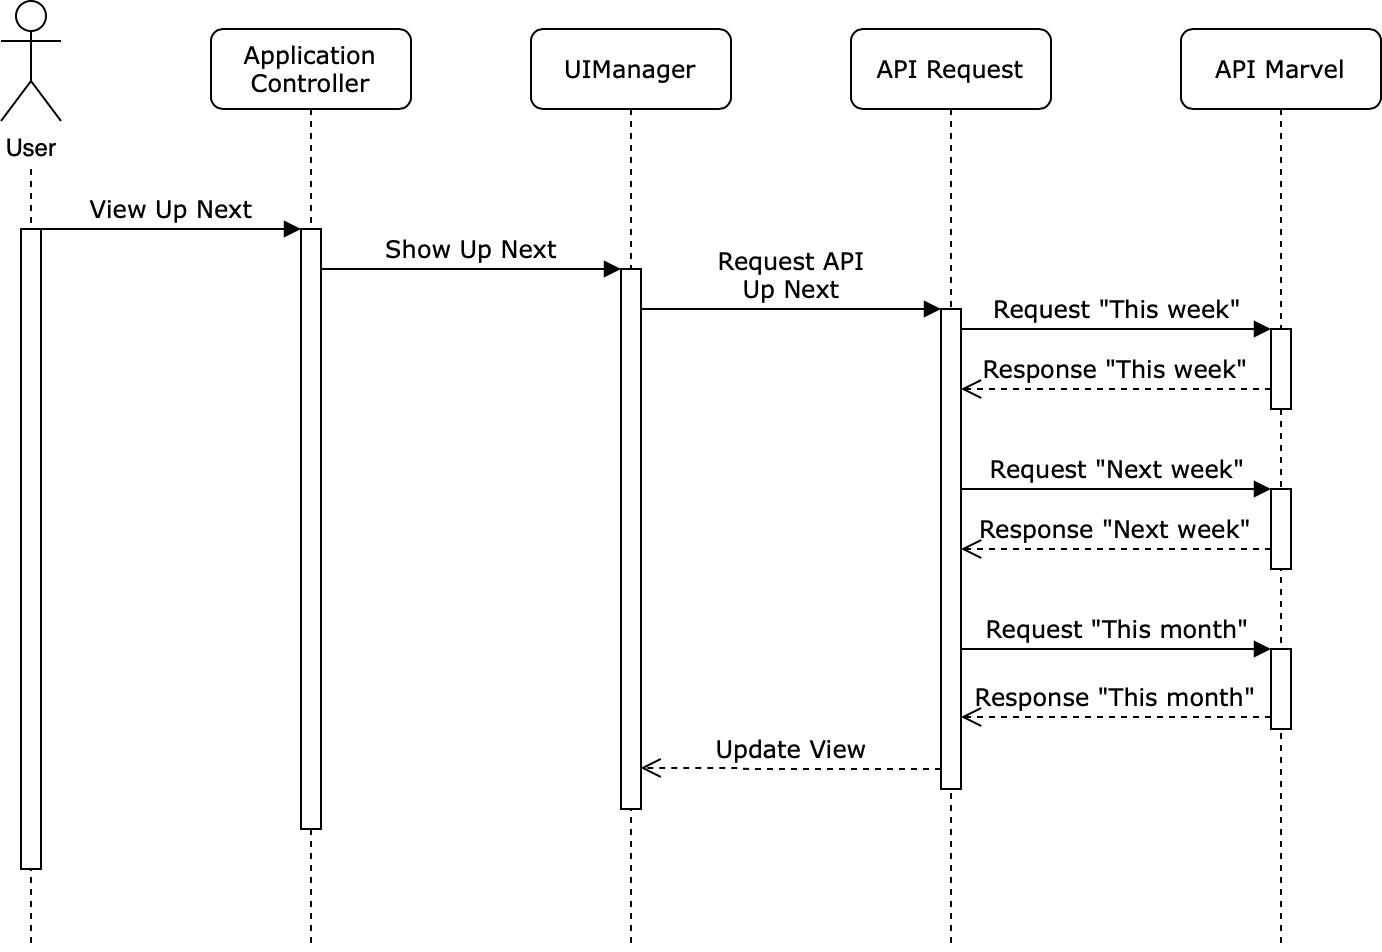
\includegraphics[width=\textwidth]{img/seqdiagrams/viewupnext}
\end{figure}

\clearpage

\subsection{View To Read}
The ”View To Read" procedure starts when the user presses the ”To Read” tab in the Tab Bar. The sequence diagram shows the normal procedure. \\
After the user activates the "To Read" tab, the application will send a request to Firebase in order to retrieve the identifiers of the next issues the user has to read. \\
Once these identifiers are obtained, the application will send a request to the "MarvelAPI" service in order to retrieve information about the issues. \\
Once this information is obtained, the Controller will create a custom UICollectionViewCell for each issue and insert them into a UICollectionView. \\
Furthermore and asynchronously, the application will download the cover of each issue to display to the user.

\vspace{5mm}

\begin{figure}[h]
\centering
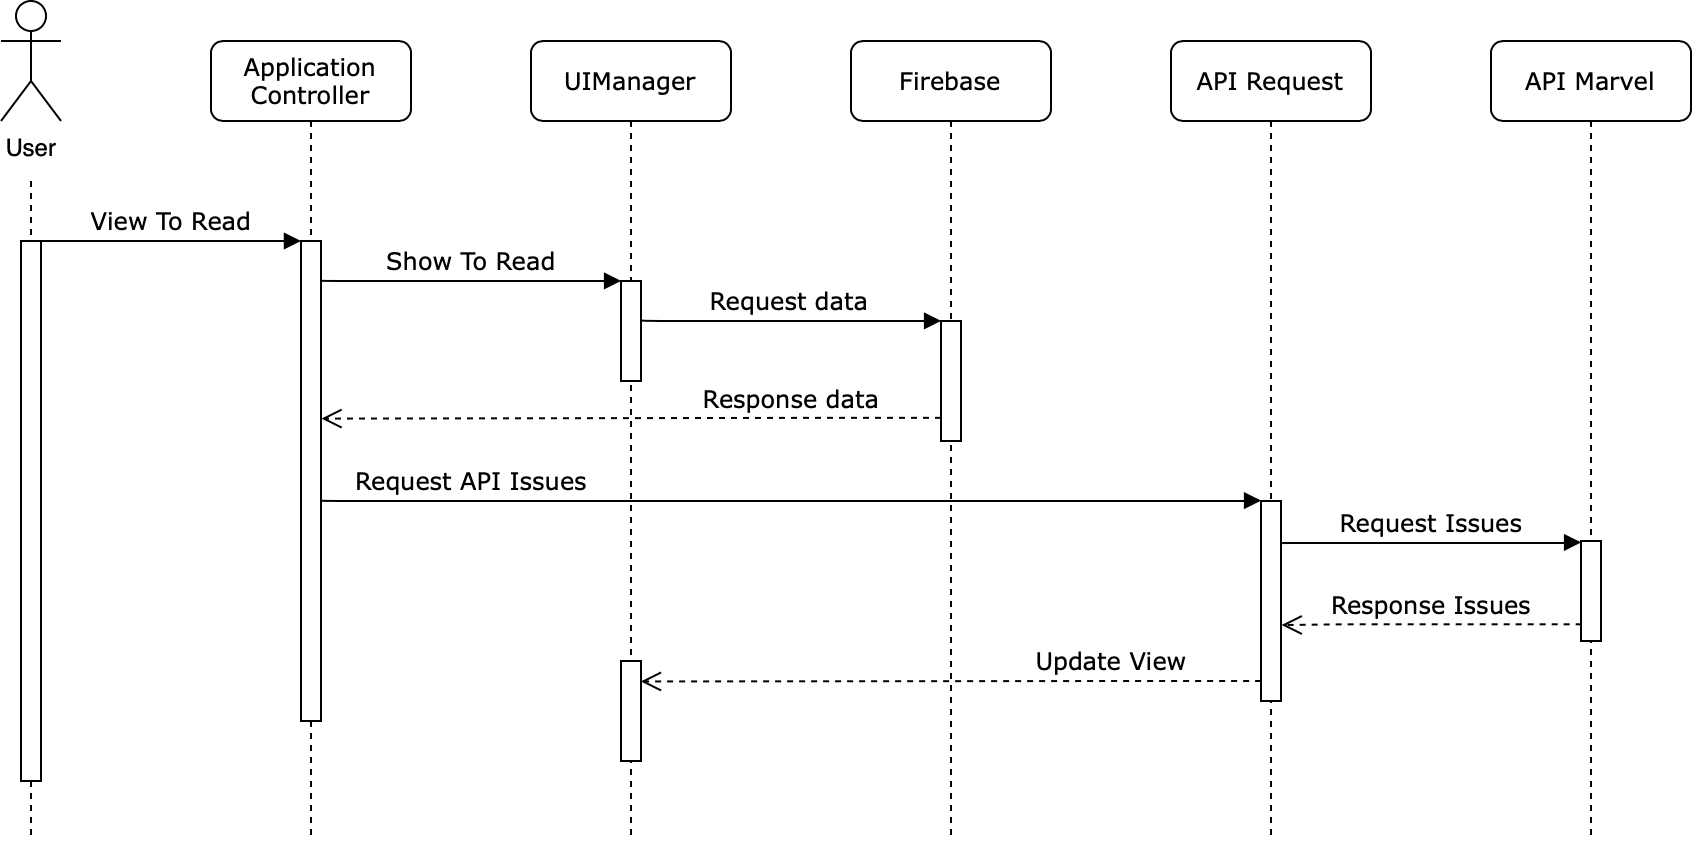
\includegraphics[width=\textwidth]{img/seqdiagrams/viewtoread}
\end{figure}

\clearpage

\subsection{View Issue}
The ”View Issue" procedure starts when the user presses a button representing an issue in one of the screens where such buttons are displayed. The sequence diagram shows the normal procedure. \\
After the user activates the "View Issue" button, the application will send a request to the "MarvelAPI" service in order to retrieve information about the issue. \\
Once this information is obtained, the Controller will create a set of UILabels, UITextViews and a UIImage to display the relevant information of the issue. 

\vspace{5mm}

\begin{figure}[h]
\centering
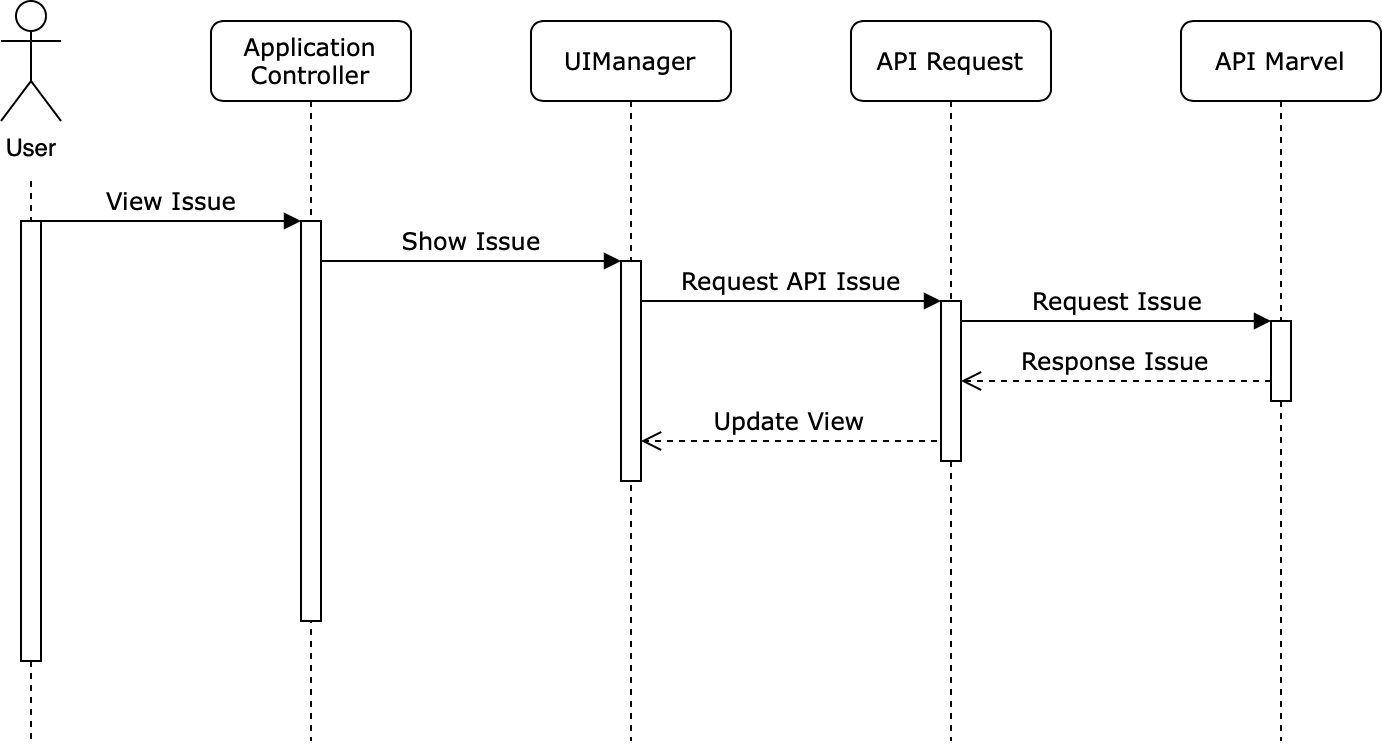
\includegraphics[width=\textwidth]{img/seqdiagrams/viewissue}
\end{figure}

\clearpage

\subsection{View Series}
The ”View Series" procedure starts when the user presses a button representing a series in one of the screens where such buttons are displayed. The sequence diagram shows the normal procedure. \\
After the user activates the "View Series" button, the application will send 1 request to the "MarvelAPI" service in order to retrieve information about the series. \\
Once all this information is obtained, the Controller will create a set of UILabels, UITextViews and a UIImage to display the relevant information of the series. 

\vspace{5mm}

\begin{figure}[h]
\centering
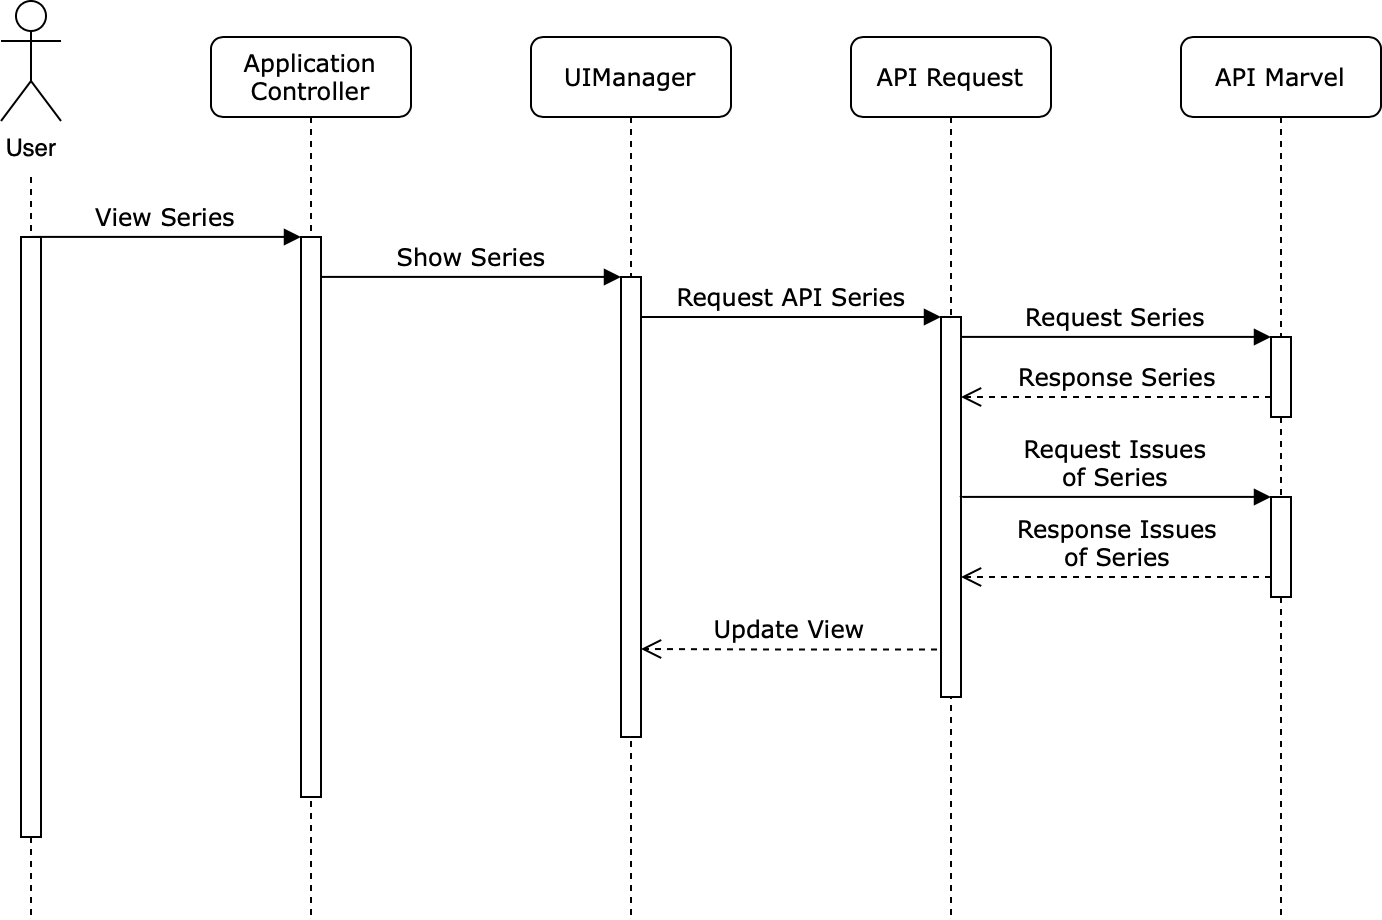
\includegraphics[width=\textwidth]{img/seqdiagrams/viewseries}
\end{figure}

\clearpage

\subsection{View Issues of Series}
The ”View Issues of Series" procedure starts when the user presses the "See all issues" button when he's viewing a series. The sequence diagram shows the normal procedure. \\
After the user activates the "See all issues" button, the application will send a request to the "MarvelAPI" service in order to retrieve all the issues belonging to that series. \\
Once all this information is obtained, the Controller will create a UITableViewCell for each issue and insert them into a UITableView, dividing them in expandable sections with 10 maximum cells for section. 

\vspace{5mm}

\begin{figure}[h]
\centering
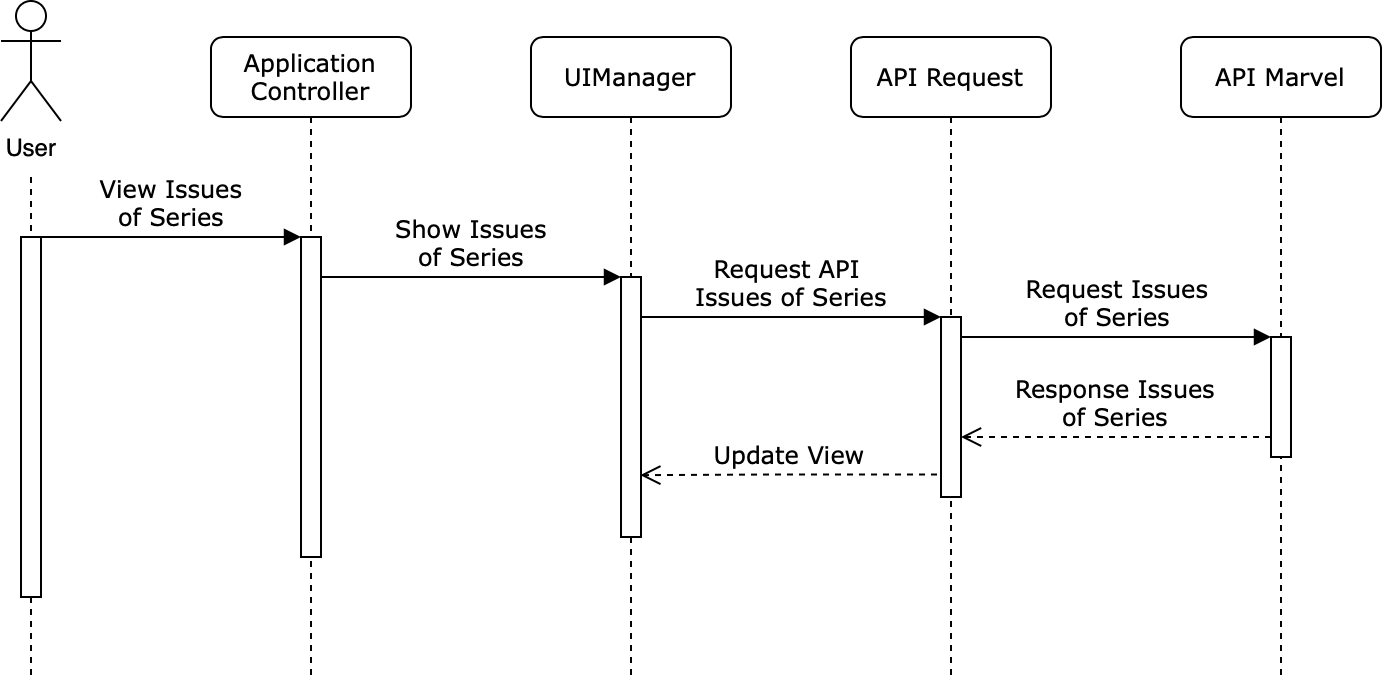
\includegraphics[width=\textwidth]{img/seqdiagrams/viewissuesofseries}
\end{figure}

\clearpage

\subsection{Mark Issue as Read}
The ”Mark Issue as Read" procedure starts when the user presses the corresponding button while he's either viewing an issue or the "To Read" section. The sequence diagram shows the normal procedure. \\
After the user activates the "Mark Issue as Read" button, the application will send a request to Firebase in order to register the issue as read in the database. \\
After receiving a notification of success, the Controller will update the GUI to show the success of the procedure. 

\vspace{5mm}

\begin{figure}[h]
\centering
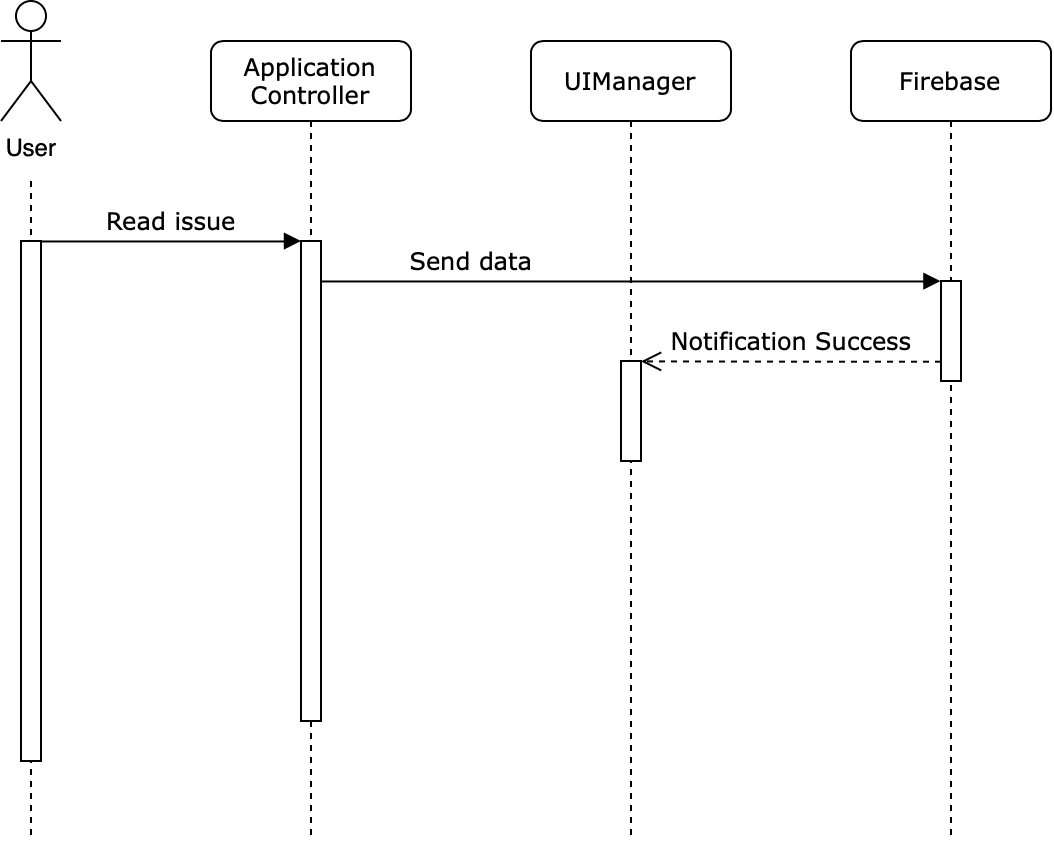
\includegraphics[width=\textwidth]{img/seqdiagrams/readissue}
\end{figure}

\clearpage

\subsection{Follow a Series}
The ”Follow a Series" procedure starts when the user presses the corresponding button while he's viewing a series. The sequence diagram shows the normal procedure. \\
After the user activates the "Follow a Series" button, the application will send a request to Firebase in order to register the series as followed in the database. \\
After receiving a notification of success, the Controller will update the GUI to show the success of the procedure. 

\vspace{5mm}

\begin{figure}[h]
\centering
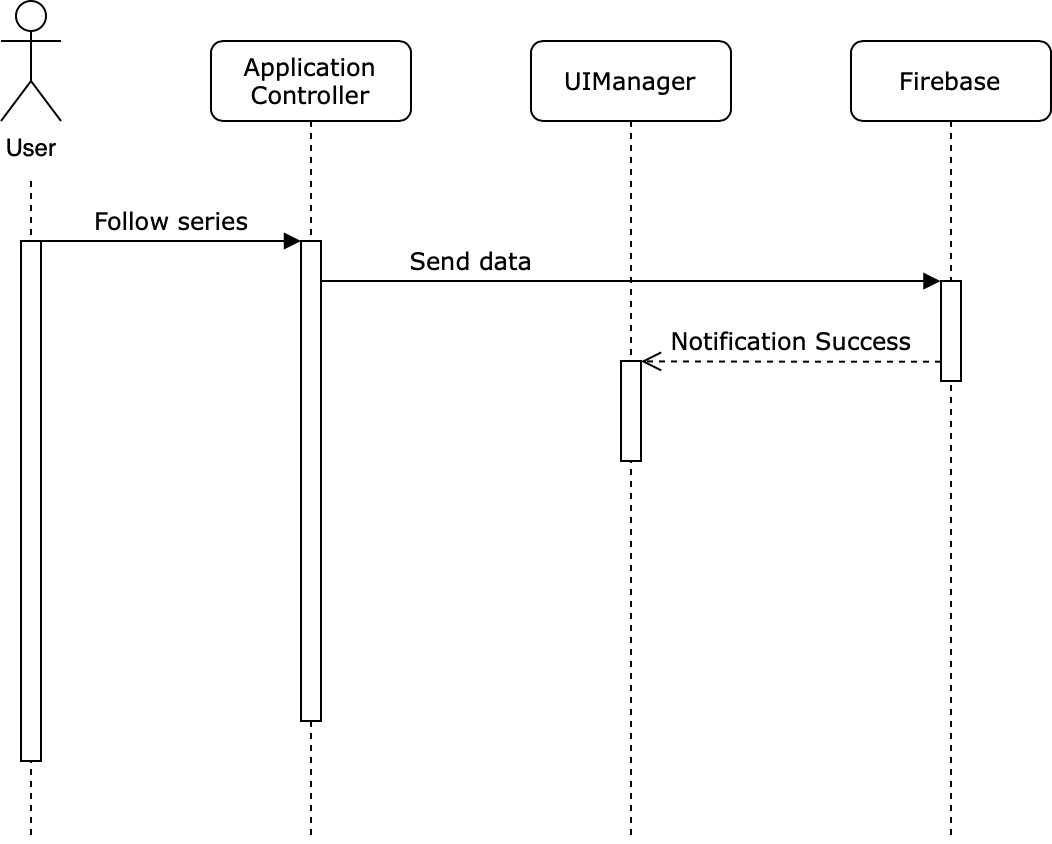
\includegraphics[width=\textwidth]{img/seqdiagrams/followseries}
\end{figure}

\clearpage

\subsection{Search a Series}
The ”Search a Series” procedure starts when the user presses the ”Search" tab in the Tab Bar. The sequence diagram shows the normal procedure. \\
After the user activates the "Search" tab, the application will send a request to the ”MarvelAPI” service in order to retrieve the series whose name matches the string written by the user. \\
Once this information is obtained, the Controller will create a UITableViewCell for each issue and insert them in a TableView. 

\vspace{5mm}

\begin{figure}[h]
\centering
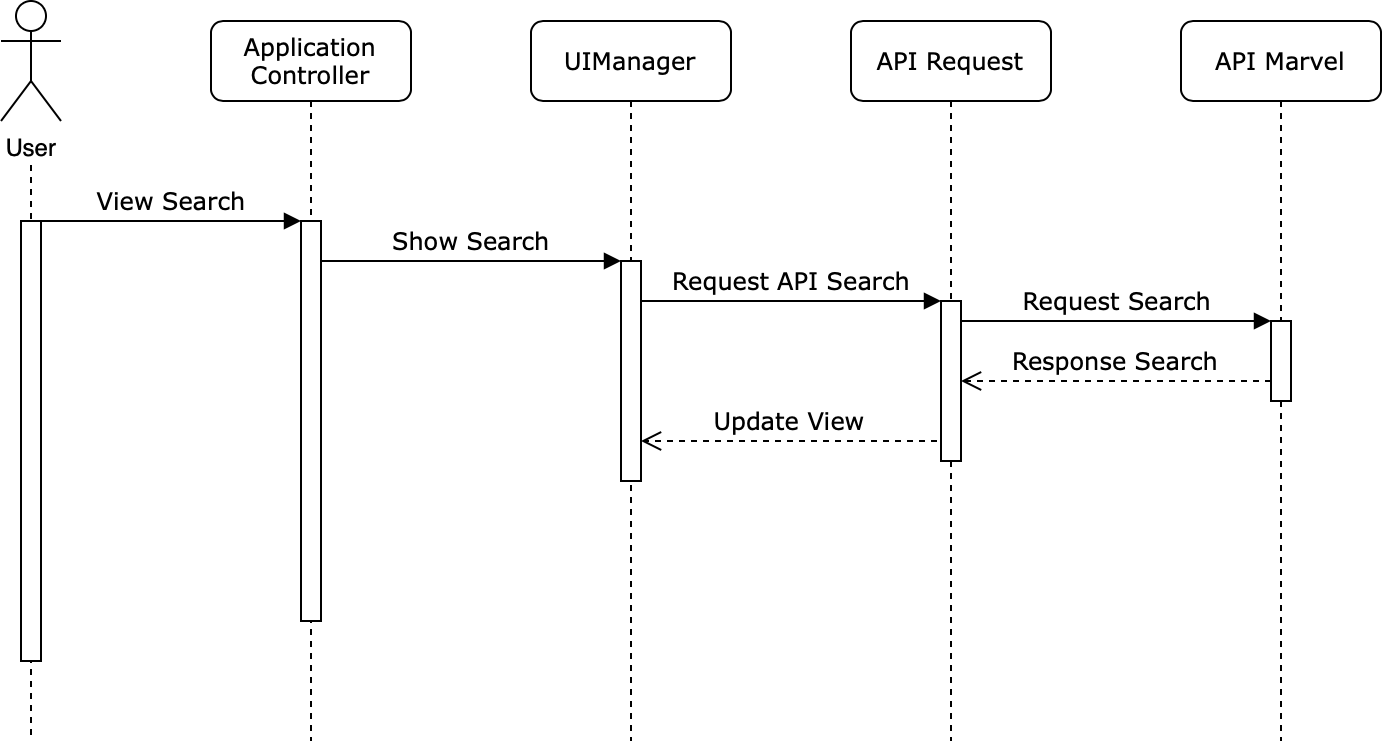
\includegraphics[width=\textwidth]{img/seqdiagrams/searchseries}
\end{figure}




%------------------------------------------------------------------------------------------------------------------------------------------------
\clearpage
{\section{User Interface Design}}
\label{sect:ui}
In this section we show the user interfaces of all the screens of the application. \newline

\vspace{28mm}

\begin{figure}[h]
  \begin{subfigure}[b]{0.4\textwidth}
    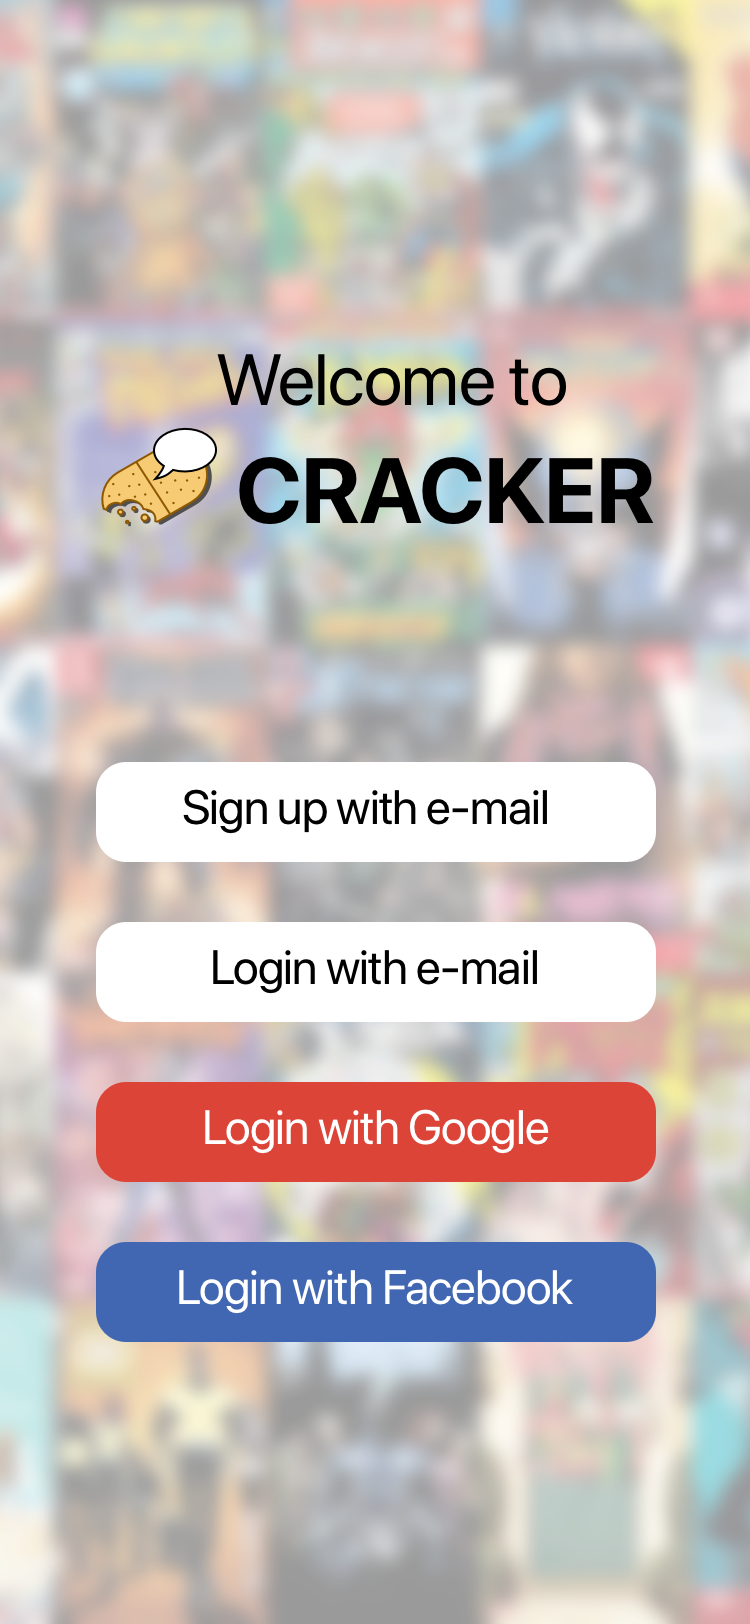
\includegraphics[width=\textwidth]{img/mockups/login}
    \caption{Login}
    \label{fig:1}
  \end{subfigure}
  \hfill
  \begin{subfigure}[b]{0.4\textwidth}
    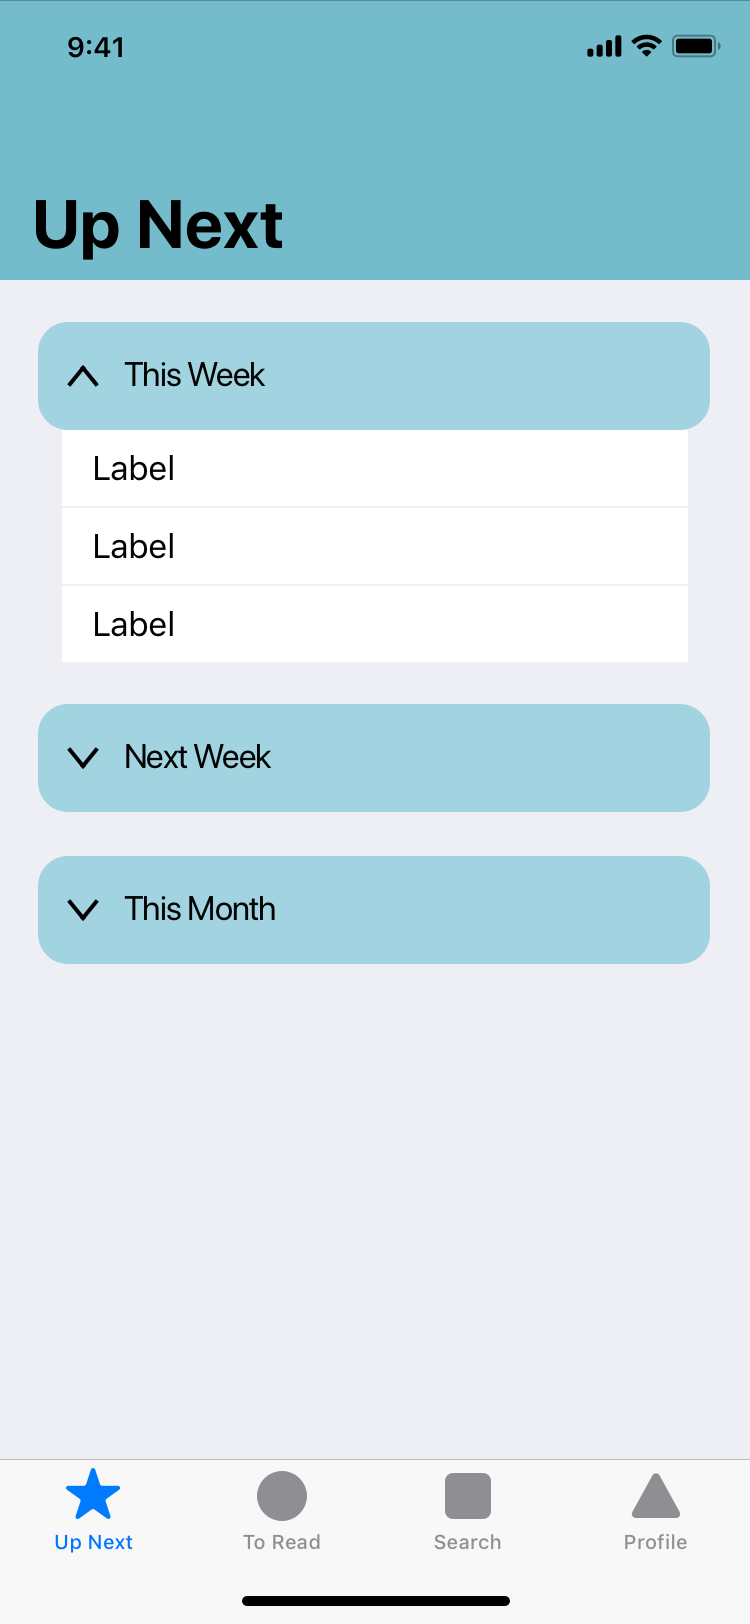
\includegraphics[width=\textwidth]{img/mockups/up_next}
    \caption{Up Next}
    \label{fig:2}
  \end{subfigure}
\end{figure}

\clearpage

\begin{figure}[p]
  \begin{subfigure}[b]{0.4\textwidth}
    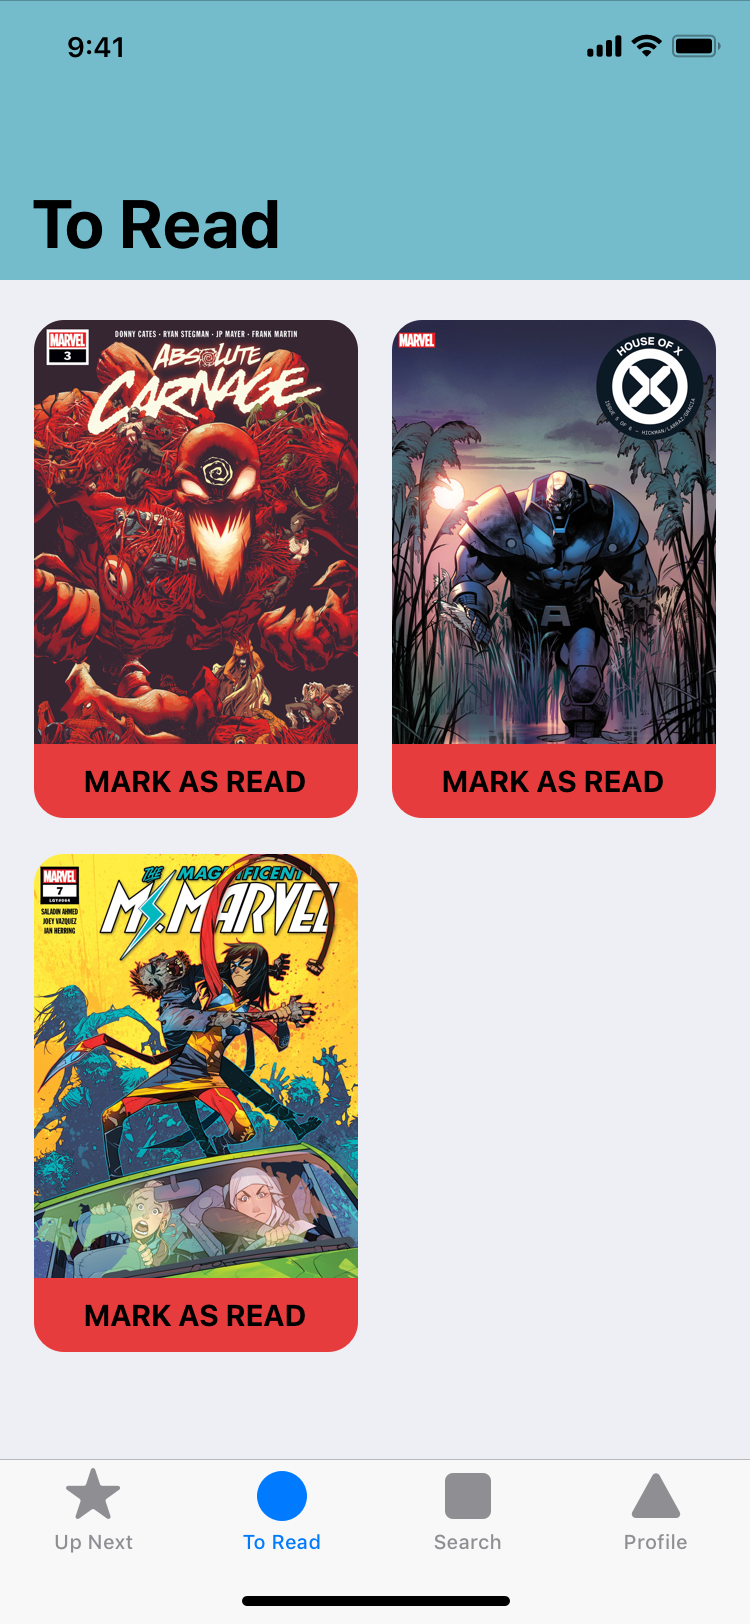
\includegraphics[width=\textwidth]{img/mockups/to_read}
    \caption{To Read}
    \label{fig:1}
  \end{subfigure}
  \hfill
  \begin{subfigure}[b]{0.4\textwidth}
    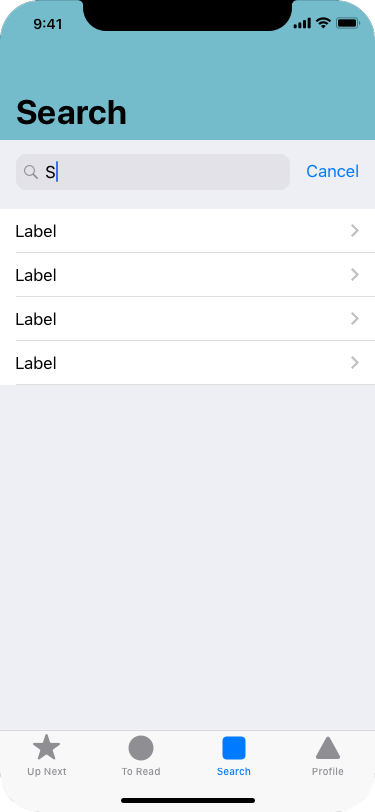
\includegraphics[width=\textwidth]{img/mockups/search}
    \caption{search}
    \label{fig:2}
  \end{subfigure}
\end{figure}

\clearpage

\begin{figure}[p]
  \begin{subfigure}[b]{0.4\textwidth}
    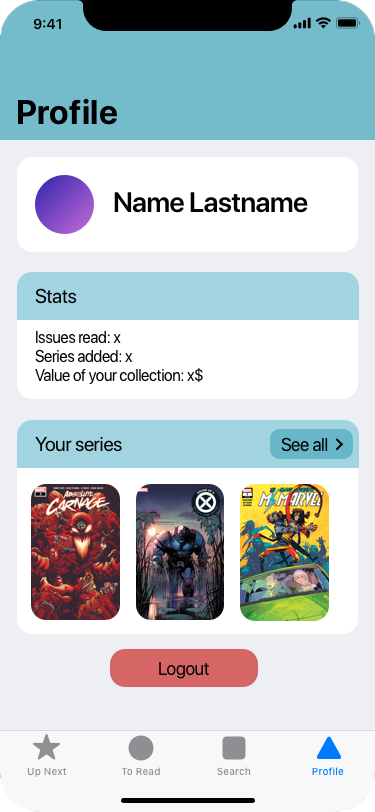
\includegraphics[width=\textwidth]{img/mockups/profile}
    \caption{Profile}
    \label{fig:1}
  \end{subfigure}
  \hfill
  \begin{subfigure}[b]{0.4\textwidth}
    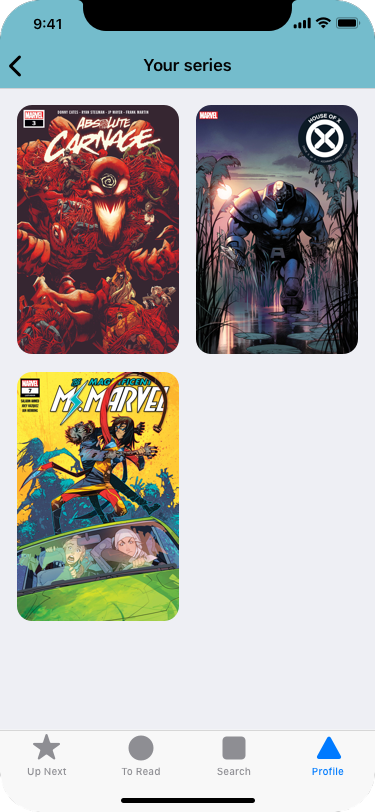
\includegraphics[width=\textwidth]{img/mockups/your_series}
    \caption{Your series}
    \label{fig:2}
  \end{subfigure}
\end{figure}

\clearpage

\begin{figure}[p]
  \begin{subfigure}[b]{0.4\textwidth}
    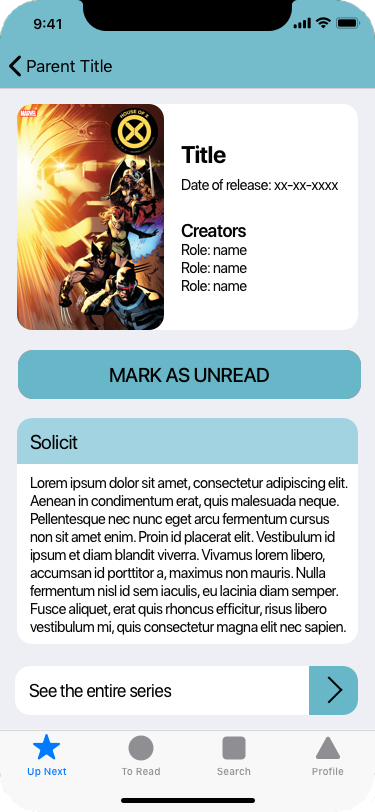
\includegraphics[width=\textwidth]{img/mockups/issue}
    \caption{Issue}
    \label{fig:1}
  \end{subfigure}
  \hfill
  \begin{subfigure}[b]{0.4\textwidth}
    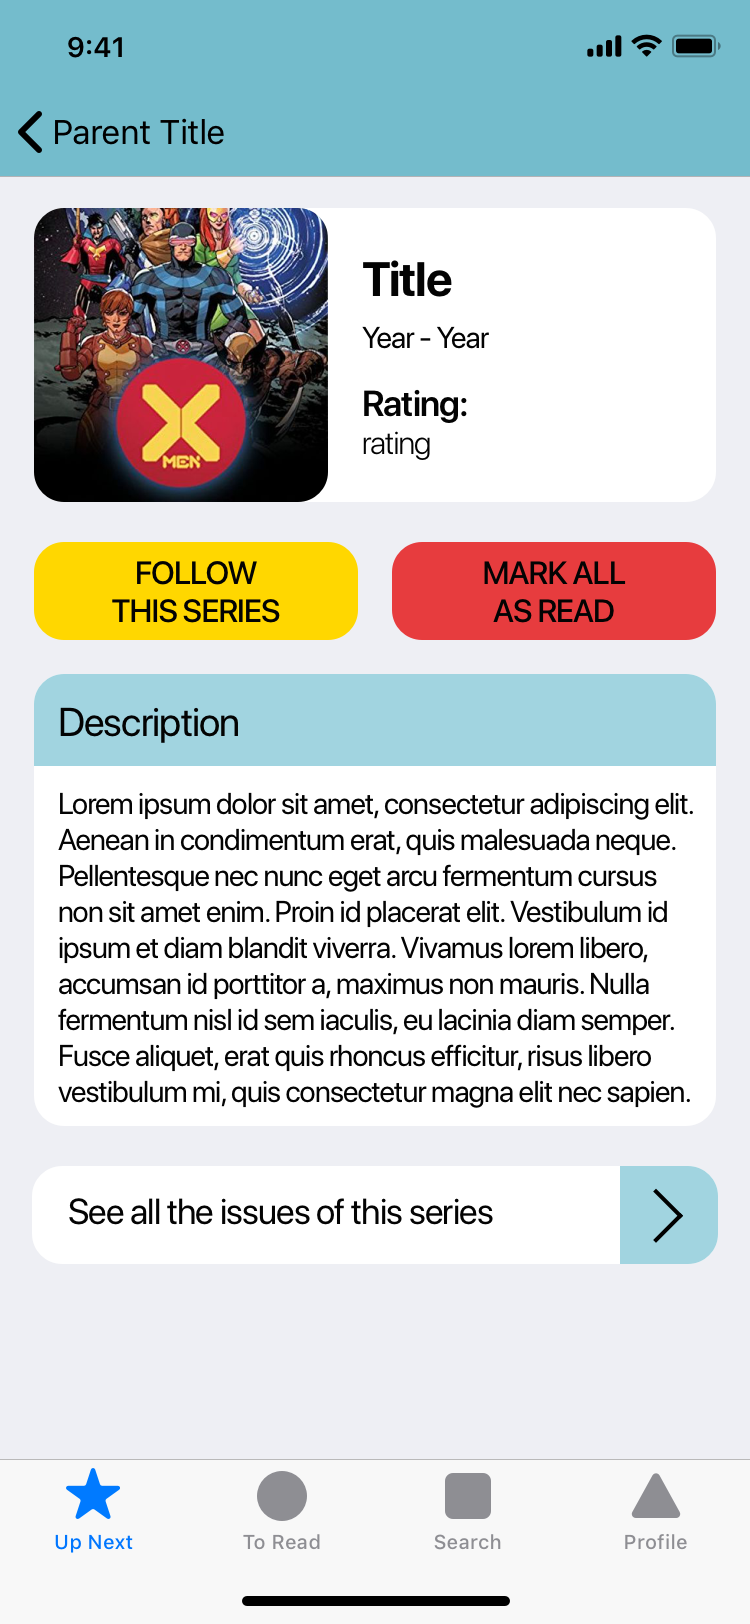
\includegraphics[width=\textwidth]{img/mockups/series}
    \caption{Series}
    \label{fig:2}
  \end{subfigure}
\end{figure}

\clearpage

\begin{figure}[p]
  \begin{subfigure}[b]{0.4\textwidth}
    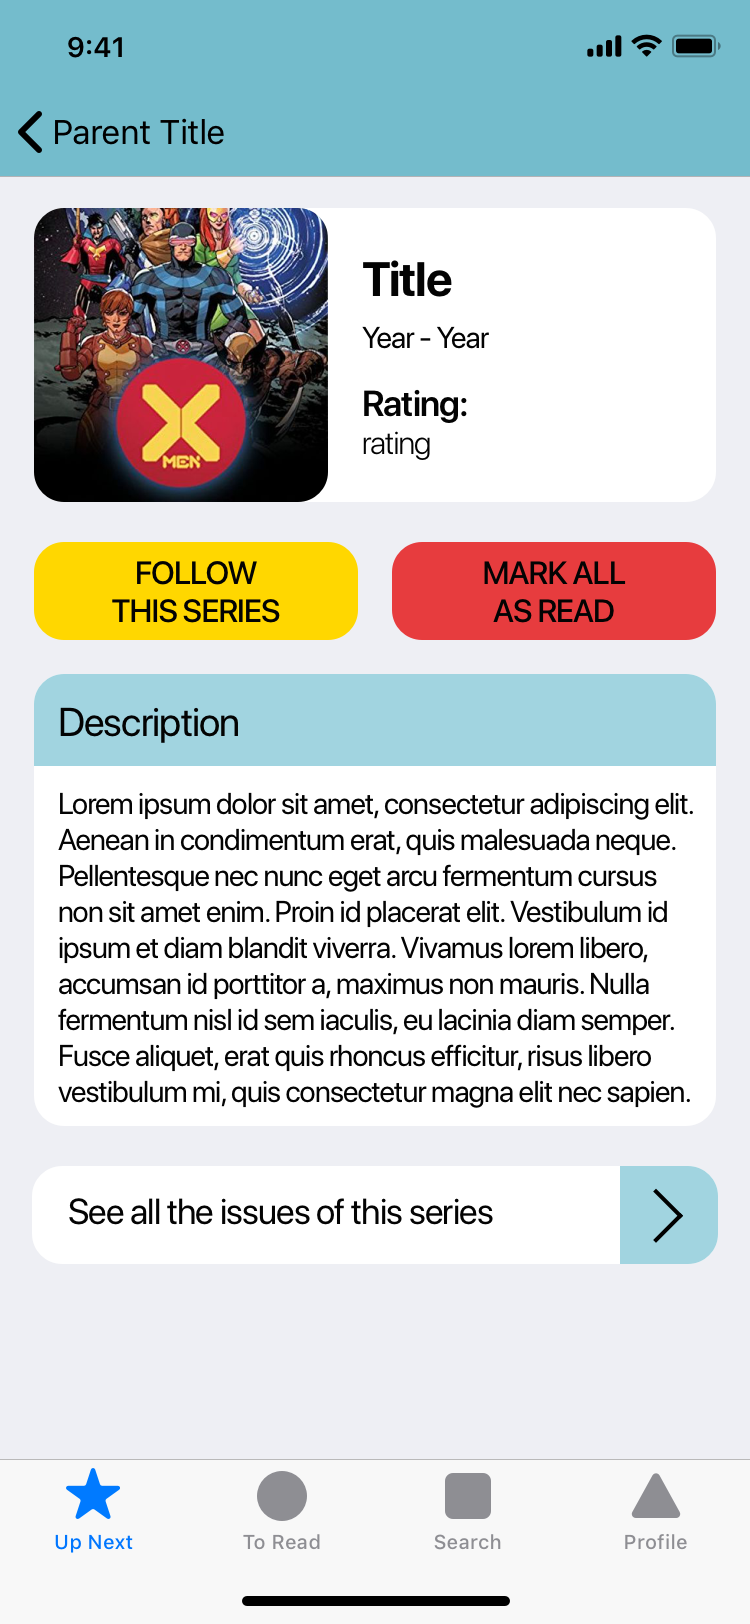
\includegraphics[width=\textwidth]{img/mockups/series}
    \caption{Series: light mode}
    \label{fig:1}
  \end{subfigure}
  \hfill
  \begin{subfigure}[b]{0.4\textwidth}
    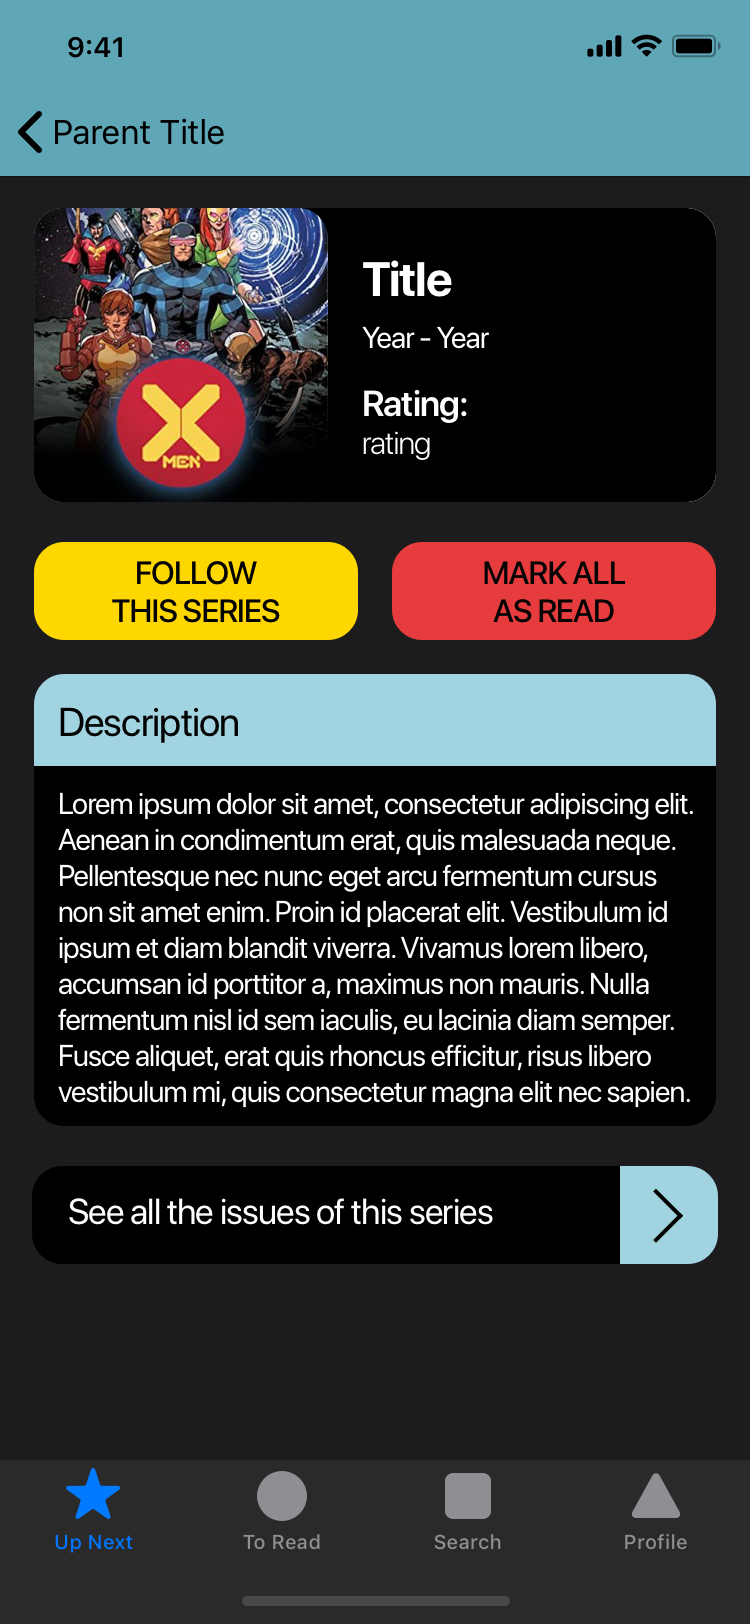
\includegraphics[width=\textwidth]{img/mockups/dark_mode}
    \caption{Series: dark mode}
    \label{fig:2}
  \end{subfigure}
\end{figure}

\clearpage

We close this section by showing the interaction between the different screens.
\vspace{8mm}

\begin{figure}[h]
\centering
\includegraphics[width=\textwidth]{img/ui_interaction}
\end{figure}



%------------------------------------------------------------------------------------------------------------------------------------------------
\clearpage
{\section{Software System Attributes}}
\label{sect:attributes}
\subsection{Reliability}
As the majority of function requires an internet connection, the software is reliable as long as there are no connectivity problems.

\subsection{Availability}
The availability parameter also relies on the internet connection signal and on the responses provided by Marvel APIs. No problems of availability were found during the development phase.

\subsection{Security}
As all the information provided are retrieved from the web, there are different checks to perform in order to keep the user information safe. Furthermore, for the communication with external services, the HTTPS protocol was chosen to guarantee greater security.


%------------------------------------------------------------------------------------------------------------------------------------------------
\clearpage
{\section{Testing}}
\label{sect:tests}
\input{sections/tests}

%------------------------------------------------------------------------------------------------------------------------------------------------
\clearpage
{\section{Used Tools}}
\label{sect:tools}
The following softwares, tools and services have been used for the development of the application:
\vspace{5mm}
\begin{itemize}
\item XCode 11.3
\item Sketch
\item Github
\item Firebase
\end{itemize}

%------------------------------------------------------------------------------------------------------------------------------------------------


\end{document}
